\documentclass{beamer}

\usepackage[mode=buildnew,subpreambles=true]{standalone}
%%%% PACKAGES

\usepackage{import}
\usepackage[toc,page]{appendix}
\usepackage[T1]{fontenc}
\usepackage[english]{babel}
\usepackage[utf8]{inputenc}
\usepackage{graphicx}
\usepackage{adjmulticol}
\usepackage[labelfont=bf]{caption}
\usepackage{float}
\usepackage{graphicx}
\usepackage{subcaption}
\usepackage{fancyhdr}
\usepackage{url}
\usepackage{amsmath} % collection de symboles mathématiques
\usepackage{amssymb} % collection de symboles mathématiques
\usepackage{amsthm}
\usepackage{bbm}
\usepackage{bm}
\usepackage{stmaryrd}
\usepackage{mathtools}
\usepackage{cancel}
\usepackage{titling}
\usepackage{nameref} % pour désigner des parties par leur nom
\usepackage{url} % pour mettre des URL
\usepackage{cite}
% \usepackage[sectionbib]{chapterbib}
% \usepackage{chapterbib}
\usepackage[numbers,sort&compress]{natbib}
% \usepackage[square,numbers,sectionbib]{natbib}
% \usepackage{bibunits}
% \usepackage{biblatex}
\usepackage{tabularx}
\usepackage{titlesec, blindtext, color}
% \usepackage{auto-pst-pdf}

%%%% TIKZ

\usepackage{pgf, tikz}
\usetikzlibrary{shapes.misc}
\usetikzlibrary{decorations.pathreplacing}

\tikzset{cross/.style={cross out, draw=black, minimum size=2*(#1-\pgflinewidth), inner sep=0pt, outer sep=0pt},
%default radius will be 1pt.
cross/.default={0.25pt},
    point/.style={
    thick,
    draw=black,
    cross out,
    inner sep=0pt,
    minimum width=4pt,
    minimum height=4pt,
    },
}

%%%% STYLE

\textheight=25 true cm
\textwidth= 20. true cm
\oddsidemargin=-1.75truecm
\evensidemargin=0.5truecm
\topmargin=-3 truecm

% \setlength{\topmargin}{-1cm}
% \setlength{\headheight}{0.43cm}
% \setlength{\headsep}{0.8cm}
% \setlength{\footskip}{0cm}
% \setlength{\textwidth}{17cm}
% \setlength{\textheight}{23.5cm}
% \setlength{\voffset}{-2.5cm}
% \setlength{\hoffset}{-0.25cm}
% \setlength{\oddsidemargin}{0cm}
% \setlength{\evensidemargin}{0cm}
\setlength{\parindent}{0pt}
\setlength{\footskip}{1.5cm}

\setlength{\droptitle}{-1cm}

\setcounter{tocdepth}{3}
\setcounter{secnumdepth}{3}

\definecolor{lcolor}{rgb}{0,0,0.6} % définition de la couleur des liens pdf
\usepackage{hyperref}
\hypersetup{pdftex,colorlinks=true,
linkcolor=lcolor,
citecolor=lcolor,
urlcolor=lcolor,
hyperindex=true,
hyperfigures=false} % fichiers pdf 'intelligents', avec des liens entre les références, etc.

\definecolor{gray75}{gray}{0.75}

\AtBeginDocument{\addtocontents{toc}{\protect\thispagestyle{empty}}}

% \titleformat{\chapter}[hang]{\vspace{-50pt}\huge\bfseries}{\thechapter\hspace{20pt}\textcolor{gray75}{|}\hspace{20pt}}{0pt}{\huge\bfseries}
\titleformat{\subsection}[block]{\hspace{0em}}{\large\textbf\thesubsection}{1em}{\large\textbf}
\titleformat{\subsubsection}[block]{\hspace{0em}}{\Small\textbf\thesubsubsection}{1em}{\Small\textbf}

\usepackage{etoolbox}
\makeatletter
\patchcmd{\@chap@pppage}{\thispagestyle{plain}}{\thispagestyle{empty}}{}{}
\makeatother

\captionsetup{font=normalsize}
\captionsetup[sub]{font=scriptsize}

%%%% COMMANDS

\providecommand{\ie}{\textit{i.e.}~}

%\renewcommand*\thesection{\arabic{section}}

\makeatletter
\providecommand*\bigcdot{\mathpalette\bigcdot@{.5}}
\providecommand*\bigcdot@[2]{\mathbin{\vcenter{\hbox{\scalebox{#2}{$\m@th#1\bullet$}}}}}
\makeatother

\providecommand{\appropto}{\mathrel{\vcenter{
  \offinterlineskip\halign{\hfil$##$\cr
    \propto\cr\noalign{\kern2pt}\sim\cr\noalign{\kern-2pt}}}}}

\providecommand\encircle[1]{%
  \tikz[baseline=(X.base)]
    \node (X) [draw, shape=circle, inner sep=0] {\strut #1};}

\providecommand\phantomarrow[2]{%
  \setbox0=\hbox{$\displaystyle #1\to$}%
  \hbox to \wd0{%
    $#2\mapstochar
     \cleaders\hbox{$\mkern-1mu\relbar\mkern-3mu$}\hfill
     \mkern-7mu\rightarrow$}%
  \,}

\providecommand{\myparagraph}[1]{\paragraph{#1}\mbox{}\\\vspace{-5pt}}

\providecommand{\isEquivTo}[1]{\underset{#1}{\sim}}

\makeatletter
\providecommand{\subalign}[1]{%
  \vcenter{%
    \Let@ \restore@math@cr \default@tag
    \baselineskip\fontdimen10 \scriptfont\tw@
    \advance\baselineskip\fontdimen12 \scriptfont\tw@
    \lineskip\thr@@\fontdimen8 \scriptfont\thr@@
    \lineskiplimit\lineskip
    \ialign{\hfil$\m@th\scriptstyle##$&$\m@th\scriptstyle{}##$\crcr
      #1\crcr
    }%
  }
}
\makeatother

% \makeatletter
% % Original \l@section:
% %\renewcommand*\l@section{\vskip 6pt plus 1pt minus 1pt
% %                         \@dottedtocline{1}{1.5em}{2.3em}}
% % Modified \l@section:
% \renewcommand*\l@section{\ifnum\c@tocdepth>\z@\vskip 6pt plus 1pt minus 1pt \fi
%                          \@dottedtocline{1}{1.5em}{2.3em}}
% \makeatother

\providecommand\smallO[1]{
      \mathchoice
         {% mode \displaystyle
            \ensuremath{\mathop{}\mathopen{}{\scriptstyle\mathcal{O}}\mathopen{}\left(#1\right)}
         }
         {% mode \textstyle
            \ensuremath{\mathop{}\mathopen{}{\scriptstyle\mathcal{O}}\mathopen{}\left(#1\right)}
         }
         {% mode \scriptstyle
            \ensuremath{\mathop{}\mathopen{}{\scriptscriptstyle\mathcal{O}}\mathopen{}\left(#1\right)}
         }
         {% mode \scriptscriptstyle
            \ensuremath{\mathop{}\mathopen{}{o}\mathopen{}\left(#1\right)}
         }
   }

%%%% PATCH

% \makeatletter
% \let\orig@document\document
% \let\orig@enddocument\enddocument
% \def\sa@document{%
%   \endgroup
%   \global\let\enddocument\sa@enddocument
%   \sa@atbegindocument
% }
% \def\sa@enddocument{%
%   \sa@atenddocument
%   \global\let\document\orig@document
%   \global\let\enddocument\orig@enddocument
%   \begingroup
%   \@ignoretrue
%   \def\@currenvir{document}%
%   \aftergroup\endinput
% }
% \makeatother


%%%%% INFORMATION

\title{Large deviations of active work in systems of active Brownian particles}
\shorttitle{Large deviations of active work in systems of ABPs}

\author{Yann-Edwin Keta}

\supervisor{Robert Jack}

\location{StatMech meeting, Department of Chemistry,\\
University of Cambridge}

\date{20/02/2020}

%%%%% DOCUMENT

\begin{document}

%% TITLE PAGE

{
\setbeamertemplate{footline}{}
\makeatletter
    \setbeamertemplate{headline}[default]
    \def\beamer@entrycode{\vspace*{-\headheight}}
\begin{frame}[noframenumbering]

\vspace*{-4mm}
{
 \hspace*{-\beamerleftmargin}%
\begin{minipage}{\paperwidth}
\includegraphics[width=\paperwidth]{header.eps}
\end{minipage}
}

\titlepage

\vspace{-20pt}
\begin{center}
\href{https://github.com/yketa/DAMTP_2019_Wiki}{\bf{\footnotesize \faGithub~ yketa/DAMTP\_2019\_Wiki}}
\end{center}

\hfill
\begin{minipage}{0.5\linewidth}
\centering
\includegraphics[scale=0.18]{cambridge.eps}
\end{minipage}
\hfill
\begin{minipage}{0.42\linewidth}
\centering
\includegraphics[scale=0.25]{enslyon.eps}
\end{minipage}
\hfill

\end{frame}
}

%% TABLE OF CONTENTS

{\footerwithoutframenumber
\begin{frame}<beamer>[noframenumbering]{Contents}
  \tableofcontents
\end{frame}
}

%% PRESENTATION

\section{Active matter}

\subsection{Non-equilibrium systems}

\begin{frame}[t]{Non-equilibrium systems}

Non-equilibrium dynamics breaks time-reversal symmetry and thus detailed balance. \pause We can identify 3 general classes:
\begin{itemize}[<+->]
  \item Systems relaxing towards equilibrium.
  \item Systems with boundary conditions imposing steady currents.
  \item Active matter.
\end{itemize}

\only<2>{
\begin{example}
Thermal system adapting to its thermostat, glasses.
\end{example}
}
\only<3>{
\begin{example}
Sheared liquid, metal rod between two thermostats.
\end{example}
}
\only<4>{
\begin{definition}
System composed of self-driven units, \textit{active particles}, each capable of converting stored or ambient free energy into systematic movement.\footfullcitenomark{marchetti2013hydrodynamics}
\end{definition}
\begin{example}
Cell tissues, swarms of bacteria, schools of fish, flocks of birds.
\end{example}
}

\footfullcitenomark{berthier2019lectures}
\footfullcitenomark{cates2015motility}

\end{frame}

\begin{frame}{Non-equilibrium phenomenon in active matter: swarming}

\begin{itemize}
  \item[$\rightarrow$] Aligning self-propelled disks with repulsive interactions (Vicsek model).
\end{itemize}
\vspace{-5pt}
\begin{align*}
\dot{\underline{r}}_i = v_0 \begin{pmatrix} \cos \theta_i \\ \sin \theta_i \end{pmatrix} - \mu \sum_{j=1}^N \nabla U_{ij},~ \dot{\theta}_i = \frac{1}{\tau} (\varphi_i - \theta_i) + \xi_i,~ \varphi_i = \arg(\dot{\underline{r}}_i)
\end{align*}

\vspace{-10pt}
\insertmovie{0.52}{vicsek.png}{vicsek.mp4}{}

\footfullcitenomark{vicsek1995novel}
\footfullcitenomark{szabo2006phase}

\end{frame}

\begin{frame}{Non-equilibrium phenomenon in active matter: MIPS}

\begin{itemize}
  \item[$\rightarrow$] Active Brownian particles with repulsive soft interactions.
\end{itemize}
\vspace{-5pt}
\begin{align*}
\dot{\underline{r}}_i = v_0 \begin{pmatrix} \cos \theta_i \\ \sin \theta_i \end{pmatrix} - \mu \sum_{j=1}^N \nabla U_{ij},~ \dot{\theta}_i = \sqrt{2 \tau^{-1}}\xi_i
\end{align*}

\vspace{-10pt}
\insertmovie{0.6}{mips.png}{mips.mov}{}

\footfullcitenomark{keta2019cooperative}

\end{frame}

\begin{frame}{Entropy production rate}

\begin{itemize}
  \item[$\rightarrow$] For $\{\underline{r}_i, \underline{u}_i\}_0^{\tau}$ a translational and orientational trajectory...
\end{itemize}

\begin{align*}
\dot{\mathcal{S}}_N\left[\{\underline{r}_i, \underline{u}_i\}_0^{\tau}\right] = \frac{1}{\tau} \log\frac{\mathcal{P}_N\left[\{\underline{r}_i, \underline{u}_i\}_0^{\tau}\right]}{\mathcal{P}_N^R\left[\{\underline{r}_i, \underline{u}_i\}_0^{\tau}\right]},
\end{align*}
\begin{align*}
\dot{\mathcal{S}}_N = \lim_{\tau \rightarrow \infty} \left<\dot{\mathcal{S}}_N\left[\{\underline{r}_i, \underline{u}_i\}_0^{\tau}\right]\right>,
\end{align*}

\return
\begin{itemize}
  \item[$\rightarrow$] ... defines a distance to equilibrium which cancels at equilibrium.
\end{itemize}
\begin{align*}
\dot{\mathcal{S}}_N\left[\{\underline{r}_i, \underline{u}_i\}_0^{\tau}\right] \propto \frac{1}{\tau} \Delta F \Rightarrow \dot{\mathcal{S}}_N = 0.
\end{align*}

\footfullcitenomark{fodor2016far}
\footfullcitenomark{nardini2017entropy}

\end{frame}

\subsection{Active Brownian particles}

\begin{frame}[t]{Active Brownian particles}

\begin{itemize}
  \item[$\rightarrow$] \only<1>{$N$}\only<2->{$\color{red}N$} ABPs with evolution
\end{itemize}
\begin{align*}
\dot{\underline{r}}_i &= - \only<1>{\mu}\only<2-5>{\textcolor{red}{\mu}}\only<6->{\frac{1}{3}\textcolor{red}{\frac{\sigma}{l_p}}} \sum_{j=1}^N \nabla U_{ij} + \only<1>{v_0}\only<2>{\textcolor{red}{v_0}} \begin{pmatrix} \cos\theta_i \\ \sin\theta_i \end{pmatrix} + \sqrt{\only<1-4>{2 \only<1>{D}\only<2-4>{\textcolor{red}{D}}} \only<5->{\frac{2}{3}\textcolor{red}{\frac{\sigma}{l_p}}} \vphantom{\frac{2}{3}\frac{\sigma}{l_p}}} \underline{\eta}_i,\\
\dot{\theta}_i &= \sqrt{2 \only<1>{D_r}\only<2-3>{\textcolor{red}{D_r}}\only<4->{\textcolor{red}{\frac{\sigma}{l_p}}} \vphantom{\frac{\sigma}{l_p}}} \xi_i,
\end{align*}
\begin{itemize}
  \item[$\rightarrow$] $U_{ij}$ $\equiv$ WCA potential, $\underline{\eta}_i$, $\xi_i$ $\equiv$ Gaussian white noises with unit variance and zero mean, \only<1-2>{$\only<2>{\color{red}}\sigma$ $\equiv$ diameter, }\only<1>{$\phi$}\only<2->{$\color{red}\phi$} $\equiv$ packing fraction.
\end{itemize}

\only<2->{
\only<2>{7}\only<3-4>{5}\only<5>{4}\only<6->{3} control parameters: $\color{red} N$, $\color{red} \phi$, \only<2>{$\color{red} \sigma$, }\only<2-5>{$\color{red} \mu$, }\only<2>{$\color{red} v_0$, }\only<2-4>{$\color{red} D$, }$\color{red} \only<2-3>{D_r}\only<4->{\frac{l_p}{\sigma} = D_r^{-1}}\vphantom{\frac{l_p}{\sigma}}$.\\
\only<3->{
\begin{itemize}
  \item[$\rightarrow$] units of space and time: $\sigma = 1$, $\sigma/v_0 = 1$
  \only<5->{\item[$\rightarrow$] Stokes-Einstein-Debye relation: $D = \frac{1}{3}D_r$}
  \only<6->{\item[$\rightarrow$] $\mu = D$}
\end{itemize}
}
}

\footfullcitenomark{nemoto2019optimizing}

\end{frame}

\begin{frame}{Active work}

\vspace{-5pt}

\begin{align*}
\dot{\mathcal{S}}_N = \lim_{\tau \rightarrow \infty} \left<\frac{1}{\tau} \log\frac{\mathcal{P}_N\left[\{\underline{r}_i, \underline{u}_i\}_0^{\tau}\right]}{\mathcal{P}_N^R\left[\{\underline{r}_i, \underline{u}_i\}_0^{\tau}\right]}\right> = 3 \frac{l_p}{\sigma} N \lim_{\tau \rightarrow \infty} \left<w_{\tau}\right>
\end{align*}
\begin{align*}
w_{\tau} &= \frac{1}{N \tau} \int_0^{\tau} \sum_{i=1}^N \dot{\underline{r}}_i(t) \cdot \underline{u}(\theta_i(t)) \, \text{d}t\\
&= \frac{1}{N \tau} \int_0^{\tau} \sum_{i=1}^N \Bigg(1 - \frac{1}{3}\frac{\sigma}{l_p} \sum_{j=1}^N \underline{u}(\theta_i) \cdot \nabla U_{ij} + \sqrt{\frac{2}{3}\frac{\sigma}{l_p}} \underline{u}(\theta_i) \cdot \underline{\eta}_i\Bigg) \, \text{d}t
\end{align*}

\pause
\return
\return
\hfill
\begin{minipage}{0.4\linewidth}
\centering
\bf Flocking
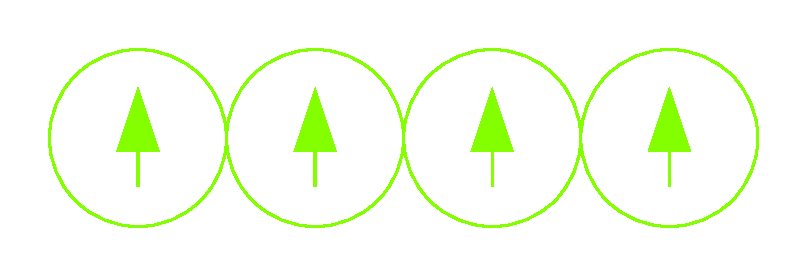
\includegraphics[width=\linewidth]{w1.eps}
$\nabla U_{ij} = 0 \Rightarrow w_{\tau} \approx 1$
\end{minipage}
\hfill
\begin{minipage}{0.4\linewidth}
\centering
\bf Jamming
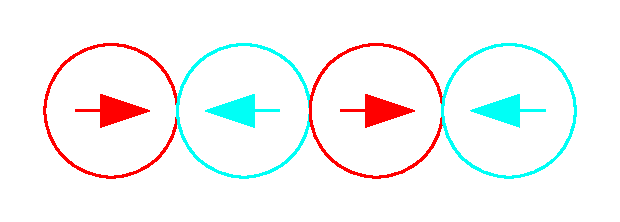
\includegraphics[width=\linewidth]{w0.eps}
$\dot{\underline{r}}_i \approx 0 \Rightarrow w_{\tau} \approx 0$
\end{minipage}
\hfill\hfill

\end{frame}

\section{Large deviation theory}

\subsection{Concepts and applications}

\begin{frame}{Large deviation principle}

\footfullcitenomark{touchette2009large}

\begin{itemize}
  \item[$\rightarrow$] $X_1, \ldots, X_n$ a sequence of random numbers and its sample average
  \begin{align*}
    S_n = \frac{1}{n} \sum_{i=1}^n X_i.
  \end{align*}
\end{itemize}

\return
\begin{align*}
S_n \text{ satisfies a LDP } \Leftrightarrow \lim_{n \rightarrow \infty} - \frac{1}{n} \log P(S_n = s) = I(s)
\end{align*}

\return
\begin{align*}
I \equiv \text{ rate function of } S_n \Leftrightarrow P(S_n = s) \asymp \exp(- n I(s))
\end{align*}

\end{frame}

\begin{frame}{LDP example: sample mean of Gaussian random variables}

\begin{itemize}
  \item[$\rightarrow$] $X_1, \ldots, X_n$ random numbers from a Gaussian distribution $(\mu, \sigma)$.
\end{itemize}

\return
\begin{align*}
S_n = \frac{1}{n} \sum_{i=1}^N X_i,
\end{align*}

\return
\begin{align*}
% P(S_n = s) &= \int_{\mathbb{R}^n} \delta(S(\underline{x}) - s) P(x_1) \ldots P(x_n) \, \text{d}\underline{x} = \sqrt{\frac{n}{2 \pi \sigma^2}} e^{-n(s - \mu)^2/(2\sigma^2)}.
P(S_n = s) = \sqrt{\frac{n}{2 \pi \sigma^2}} e^{-n(s - \mu)^2/(2\sigma^2)}.
\end{align*}

\return
\begin{align*}
\lim_{n \rightarrow \infty} - \frac{1}{n} \log P(S_n = s) = (s - \mu)^2/(2\sigma^2) = I(s).
\end{align*}
\begin{itemize}
\item[$\Rightarrow$] $S_n$ satisfies a large deviation principle.
\end{itemize}

\end{frame}

\begin{frame}[t]{LDP example: mean of random bits}

\begin{itemize}
  \item[$\rightarrow$] $B_1, \ldots, B_n$ random bits, taking value $0$ or $1$ with equal probability.
\end{itemize}

\begin{align*}
R_n = \frac{1}{n} \sum_{i=1}^n B_i
\end{align*}
\begin{align*}
P(R_n = r) \asymp \exp(- n I(r)),~ I(r) = \log 2 + r \log r + (1 - r) \log(1 - r).
\end{align*}

\only<1>{
\begin{figure}
\centering
\includegraphics[width=0.7\textwidth]{bits.eps}
\end{figure}
}

\only<2>{
\begin{figure}
\centering
\includegraphics[width=0.7\textwidth]{bits_CLT.eps}
\end{figure}

\begin{itemize}
  \item[$\rightarrow$] Deviations from the Gaussian fluctuations predicted by the Central Limit Theorem $\Rightarrow$ \textit{large} deviations.
\end{itemize}
}

\end{frame}

\begin{frame}{Gärtner-Ellis theorem}

\textit{Scaled cumulant generating function} (SCGF)
\begin{align*}
\lambda(k) = \lim_{n \rightarrow \infty} \frac{1}{n} \log \int e^{n k a} P(A_n = a) \, \text{d}a = \lim_{n \rightarrow \infty} \frac{1}{n} \log \left<e^{n k A_n}\right>.
\end{align*}

\return
\begin{align*}
\lambda \text{ is differentiable } \Rightarrow I(a) = \sup_k \left\{k a - \lambda(k)\right\} = k(a) a - \lambda(k(a)) % Legendre transform
\end{align*}

\begin{figure}
\centering
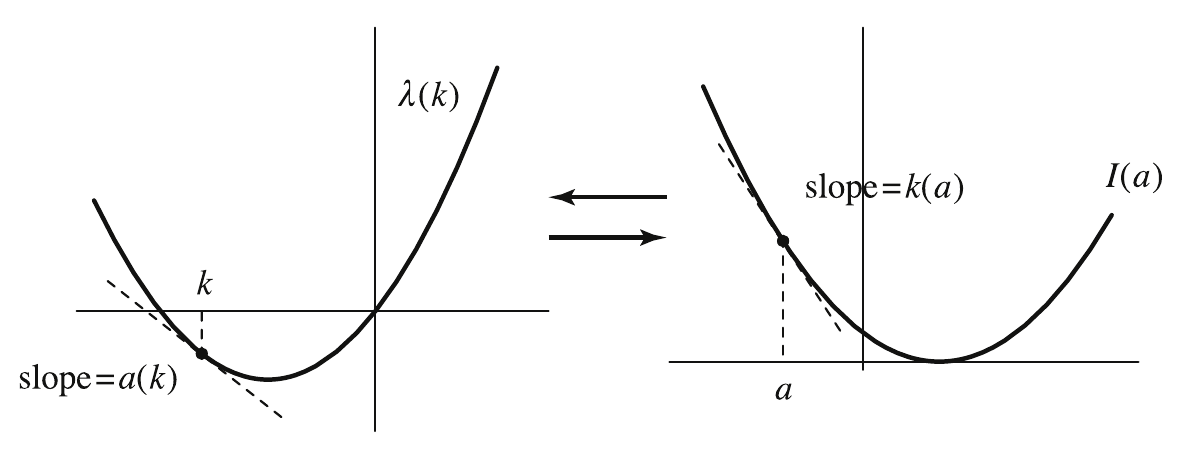
\includegraphics[width=0.6\textwidth]{Touchette_2009_fig4b.png}
\caption{\FigureFrom{touchette2009large}{}}
\end{figure}

\end{frame}

\begin{frame}{Analogy with equilibrium statistical mechanics: free energy}

\begin{align*}
E_n \equiv\text{energy of $n$ particles} \Rightarrow P_{\beta}(\omega) = \frac{e^{- \beta n E_n(\omega)}}{Z_n(\beta)} \equiv \text{Boltzmann distribution}
\end{align*}

\return
\begin{align*}
\psi(\Delta\beta) &= \lim_{n \rightarrow \infty} \frac{1}{n} \log \int e^{\Delta\beta n E_n(\omega)} P_{\beta}(\omega) \, \text{d}\omega = \lim_{n \rightarrow \infty} \frac{1}{n} \log \frac{Z_n(\beta - \Delta\beta)}{Z_n(\beta)}\\
&= \beta F(\beta) - (\beta - \Delta\beta) F(\beta - \Delta\beta)
\end{align*}
\begin{align*}
F(\beta) = -\frac{1}{\beta} \lim_{n \rightarrow \infty} \frac{1}{n} \log Z_n(\beta) \equiv \text{free energy density}
\end{align*}

\end{frame}

\begin{frame}{Analogy with equilibrium statistical mechanics: entropy}

\begin{align*}
\psi \text{ is differentiable}\xRightarrow[\text{Gärtner-Ellis}]{} P_{\beta}(E_n) \asymp \exp(-n I_{\beta}(E_n))
\end{align*}

\return
\begin{align*}
P_{\beta}(E_n) \asymp \exp(n(\underbrace{s(E_n)}_{\mathclap{\substack{\text{entropy}\\\equiv\text{number of states}}}} - \overbrace{\beta E_n}^{\mathclap{\substack{\text{Boltzmann}\\\text{function}}}} + \underbrace{\beta F(\beta)}_{\mathclap{\substack{\text{partition}\\\text{function}}}}))
\end{align*}
\begin{align*}
I_{\beta}(E_n) = -s(E_n) - \beta E_n + \beta F(\beta)
\end{align*}

\return
\begin{align*}
I_{\beta}(E_n) = 0 \Leftrightarrow F(\beta) = E_n - \frac{1}{\beta} s(E_n)
\end{align*}

\end{frame}

% \begin{frame}{Application to equilibrium statistical mechanics: microcanonical entropy}
%
% \begin{itemize}
%   \item[$\rightarrow$] $E_n$ $\equiv$ mean energy of $n$ particles.
% \end{itemize}
%
% \return
% \begin{align*}
% P(\text{d}^n\underline{\omega}) = \frac{\text{d}^n\underline{\omega}}{|\Lambda|^n} \Rightarrow P(E_n = u) = \int_{\{\underline{\omega} \in \Lambda^n : E_n(\underline{\omega}) = u\}} \frac{\text{d}^n\underline{\omega}}{|\Lambda|^n} = \frac{\Omega(E_n = u)}{|\Lambda|^n}
% \end{align*}
%
% \return
% \begin{align*}
% I(u) = \lim_{n \rightarrow \infty} -\frac{1}{n} \log P(E_n = u) = \log |\Lambda| - s(u)
% \end{align*}
%
% \return
% \begin{align*}
% s(u) = \lim_{n \rightarrow \infty} \frac{1}{n} \log \Omega(E_n = u) \equiv \text{\it microcanonical entropy density}
% \end{align*}
%
% \end{frame}
%
% \begin{frame}{Application to equilibrium statistical mechanics: canonical free energy}
%
% \begin{itemize}
%   \item[$\rightarrow$] $E_n$ $\equiv$ mean energy of $n$ particles.
% \end{itemize}
%
% \return
% \begin{align*}
% \psi(s) = \lim_{n \rightarrow \infty} \frac{1}{n} \log \int_{\Lambda^n} e^{n s E_n(\underline{\omega})} \, \frac{\text{d}^n\underline{\omega}}{|\Lambda|^n} = - \log |\Lambda| + \lim_{n \rightarrow \infty} \frac{1}{n} \log \underbrace{\int_{\Lambda^N} e^{n s E_n(\underline{\omega})} \, \text{d}\underline{\omega}}_{Z_n(-s)}
% \end{align*}
% % we recognise $Z_n$ the $n$-particle \textit{partition function}
%
% \return
% \begin{align*}
% \psi(s) = -\left.\phi(\beta)\right|_{\beta = -s} - \log |\Lambda|
% \end{align*}
%
% \return
% \begin{align*}
% \phi(\beta) = \lim_{n \rightarrow \infty} - \frac{1}{n} \log Z_n(\beta) \equiv \text{\it canonical free energy density}
% \end{align*}
%
% \end{frame}

\begin{frame}{Application to trajectories: dynamical phase transitions}

\begin{itemize}
  \item[$\rightarrow$] $d$-dimensional system of size $N$, quantities $a_i(t)$ over trajectories.
\end{itemize}

\begin{align*}
A_{N \tau} = \frac{1}{N \tau} \int_0^{\tau} \sum_{i=1}^N a_i(t) \, \text{d}t
\end{align*}
\begin{align*}
I_N(a) = \lim_{\tau \rightarrow \infty} -\frac{1}{\tau} \log P(A_{\tau} = a),~ \psi_N(s) = \lim_{\tau \rightarrow \infty} \frac{1}{\tau} \log \left<e^{s N \tau A_{\tau}}\right>
\end{align*}

\return
\begin{table}
\begin{tabular}{c | c}
\rowcolor{CaLightPink}
\bf Quantity & \bf Equilibrium counterpart\\
\hline \hline
\rowcolor{white!90!CaLightPink}
$a_i$ & Microstates of $(d+1)$-dimensional system\\
\rowcolor{white!80!CaLightPink}
$A_{N\tau}$ & Mean energy\\
\rowcolor{white!90!CaLightPink}
$s$ & Inverse temperature (conjugate to the energy)\\
\rowcolor{white!80!CaLightPink}
$\psi_N$ & Free energy difference\\
\rowcolor{white!90!CaLightPink}
$I_N$ & $-s(E_n) - \beta E_n + \beta F(\beta)$
\end{tabular}
\end{table}

\pause
\return
\begin{itemize}
  \item[$\Rightarrow$] Singularities in $I_N/N$ and $\psi_N/N$ in the limit $\tau \rightarrow \infty$ and $N \rightarrow \infty$ $\Rightarrow$ \textit{dynamical phase transitions}.
\end{itemize}

\end{frame}

\subsection{Cloning algorithm}

\begin{frame}{Cloning algorithm}

\vspace{-10pt}
\begin{align*}
Z_{\tau}(s) = \left<e^{s N \tau A_{N\tau}}\right> \equiv \begin{split}&\text{{\it dynamical} partition function}\\ &\text{of a Boltzmann-like measure}\end{split}
\end{align*}
\begin{itemize}
  \item[$\rightarrow$] $s \neq 0$ $\Rightarrow$ average dominated by trajectories with rare events.
\end{itemize}

\pause
\begin{itemize}
  \item[$\Rightarrow$] \textit{Cloning algorithm} to generate the biased measure.
\end{itemize}

\begin{figure}
\centering
\includegraphics[width=0.45\textwidth]{Nemoto_2016_fig1a.png}
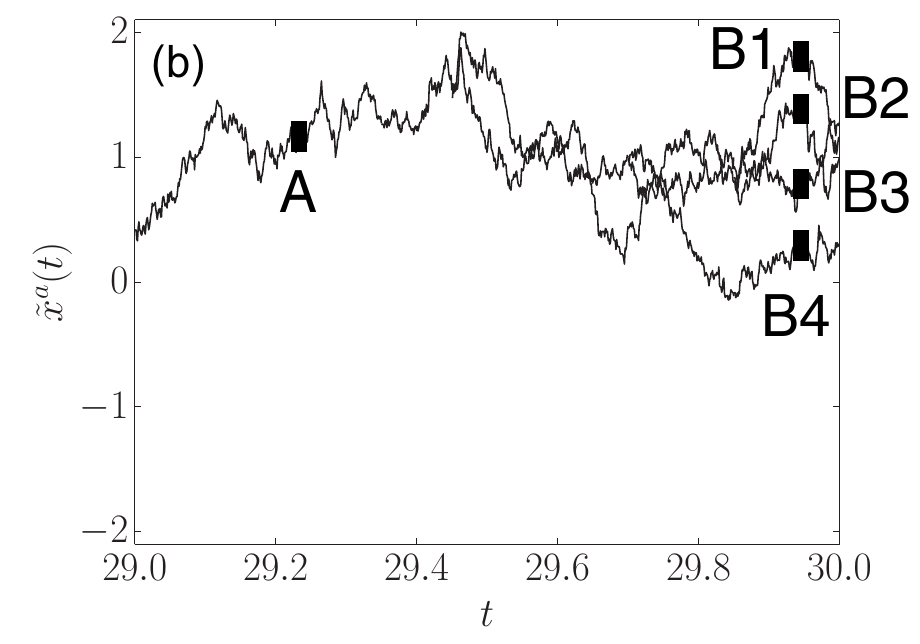
\includegraphics[width=0.45\textwidth]{Nemoto_2016_fig1b.png}
\caption{$Z_{\tau}(s) = \left<\exp\left(s \int_0^{\tau} x(t)(1 + x(t)) \, \text{d}t\right)\right>$. \FigureFrom{nemoto2016population}{}}
\end{figure}

\end{frame}

\section{Large deviations of active work}

\subsection{PSA and CM transitions}

\begin{frame}{Method}

How does the active work (\textit{i.e.} dissipation) control emerging behaviours?

\return
\begin{itemize}
  \item[$\Rightarrow$] Cloning algorithm $\rightarrow$ generate trajectories of systems of ABPs where large deviations of the active work are typical.\pause
  \begin{itemize}
    \item[$\rightarrow$] Compute SCGF...
    \begin{align*}
      \psi_N(s, \tau) = \frac{1}{\tau} \log\left<e^{- s N \tau w_{\tau}}\right>,
    \end{align*}
    \begin{align*}
      s > 0 \Leftrightarrow \text{large {\bf negative} fluctuations of } w(s)
    \end{align*}
    ... biased average of the active work...
    \begin{align*}
      w(s) = \left<w\right>_s = - \psi_N^{\prime}(s)/N,
    \end{align*}
    ... and rate function.
    \begin{align*}
      I_N(w) = \sup_s \left\{- s N w - \psi_N(s)\right\} = - s(w) N w - \psi_N(s(w)).
    \end{align*}
    \pause
    \item[$\rightarrow$] Look for singularities in $I_N/N$ and $\psi_N/N$ $\Rightarrow$ fundamental changes in the mechanisms to produce the associated fluctuations of the active work.
  \end{itemize}
\end{itemize}

\end{frame}

\begin{frame}{Unbiased behaviour}

\insertmovie{0.6}{Nemoto_2019_unbiased.png}{Nemoto_2019_unbiased.mp4}{
Unbiased trajectory for $\phi = 0.65$, $l_p/\sigma = 40$. \FigureFrom{nemoto2019optimizing}{}
}

% \begin{itemize}
%   \item[$\rightarrow$] macroscopically phase separated system with a motile cluster
% \end{itemize}

\end{frame}

\begin{frame}{PSA and CM transitions: qualitative observations}

\begin{figure}
\begin{minipage}{0.48\linewidth}
\centering
\bf CM
\Movie{1}{Nemoto_2019_CM.png}{Nemoto_2019_CM.mp4}
\end{minipage}
\hfill
\begin{minipage}{0.48\linewidth}
\centering
\bf PSA
\Movie{1}{Nemoto_2019_PSA.png}{Nemoto_2019_PSA.mp4}
\end{minipage}
\hfill\hfill
\caption{\textit{(Movie)} Biased trajectories for $N = 64$, $\phi = 0.65$, $l_p/\sigma = 40$. {\bf (left)} $s = -3.2$. {\bf (right)} $s = 0.8$. \FigureFrom{nemoto2019optimizing}{}}
\end{figure}

% \begin{itemize}
%   \only<1>{
%   \item[$\rightarrow$] large \textbf{positive} fluctuations of $w$ are associated with a directional alignment (symmetry breaking) of particles in order to avoid collisions and cancel interparticle forces $\Rightarrow$ \textit{collectively moving} (CM) state
%   }
%   \only<2>{
%   \item[$\rightarrow$] large \textbf{negative} fluctuations of $w$ are associated with the formation of a dense cluster with inward facing particles at the boundary in order to stop the movement $\Rightarrow$ \textit{phase separated arrest} (PSA)
%   }
%   \only<3>{
%   \item[$\Rightarrow$] behaviours previously observed in different physical systems can now be observed in single one when looking at the large deviations of a well chosen quantity
%   }
% \end{itemize}

\end{frame}

\begin{frame}{PSA and CM transitions: quantitative observations}

\begin{figure}
\centering
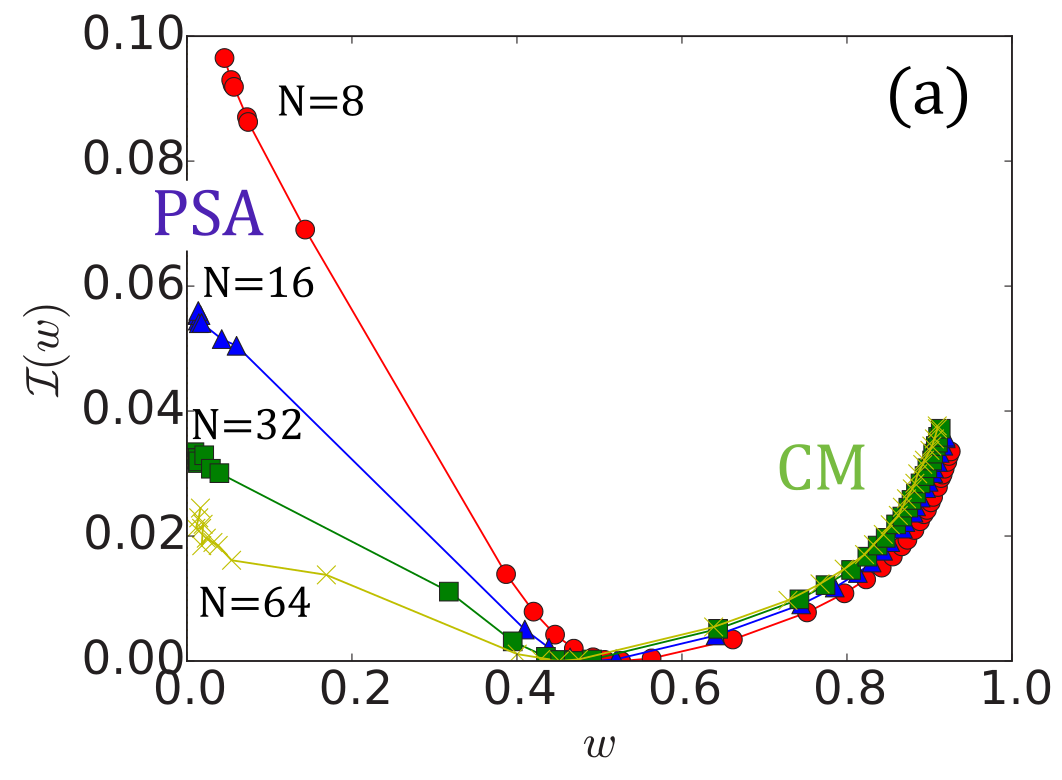
\includegraphics[width=0.49\textwidth]{Nemoto_2019_fig1a.png}
\hfill
\includegraphics[width=0.49\textwidth]{Nemoto_2019_fig1b.png}
\caption{{\bf (a)} Rescaled rate function $\mathcal{I} = I_N/N$. {\bf (b)} Biased average of active work $w(s) = \left<w\right>_s$. $\phi = 0.65$, $l_p/\sigma = 40$. \FigureFrom{nemoto2019optimizing}{}}
\end{figure}

% \begin{itemize}
%   \item[$\rightarrow$] Authors argue that the PSA transition is characterised by a discontinous jump in $w(s) = -\psi^{\prime}(s)/N$ at $s = 0$ in the limit $N \rightarrow \infty$ $\Rightarrow$ 1\textsuperscript{st} order transition.
%   \item[$\rightarrow$] On the contrary, the CM transition seems to be accompanied by a continuous jump to higher $w$.
% \end{itemize}

\end{frame}

\begin{frame}{Analysis of the CM transition}

\vspace{-10pt}
\begin{align*}
\hat{\nu} =\left|\frac{1}{N} \sum_{i=1}^N \underline{u}_i\right| \equiv \text{global order parameter},~ \nu_{\tau} = \frac{1}{\tau} \int_0^{\tau} \hat{\nu}(t) \, \text{d}t
\end{align*}

\begin{figure}
\centering
\includegraphics[width=0.60\textwidth]{Nemoto_2019_fig2a.png}
\caption{Biased average of global order parameter $\nu(s) = \left<\nu\right>_s$. $\phi = 0.65$, $l_p/\sigma = 40$. \FigureFrom{nemoto2019optimizing}{}}
\end{figure}

% \begin{itemize}
%   \only<1>{
%   \item[$\rightarrow$] We observe no coupling between orientations for $s > 0$, consistently with $\nu \rightarrow 0$ in the limit $N \rightarrow \infty$, while a finite global order remains at $s < 0$ after taking this limit.
%   }
%   \only<2>{
%   \item[$\rightarrow$] We observe $I(w) \approx J(\nu^*(w))$ for $w > \left<w\right>_0$ $\Rightarrow$ probability cost to create a large positive fluctuation of the active work is dominated by the cost to create an improbable global orientation.
%   }
% \end{itemize}

\end{frame}

\begin{frame}{Limits to this characterisation}

Two limits to this study of the CM transition:
\begin{description}
  \item[(1)] Only two high persistence lengths have been considered.
  \item[(2)] No claim on the locus of the CM transition.
\end{description}

\begin{figure}
\centering
\includegraphics[width=0.49\textwidth]{Nemoto_2019_fig2a.png}
\hfill
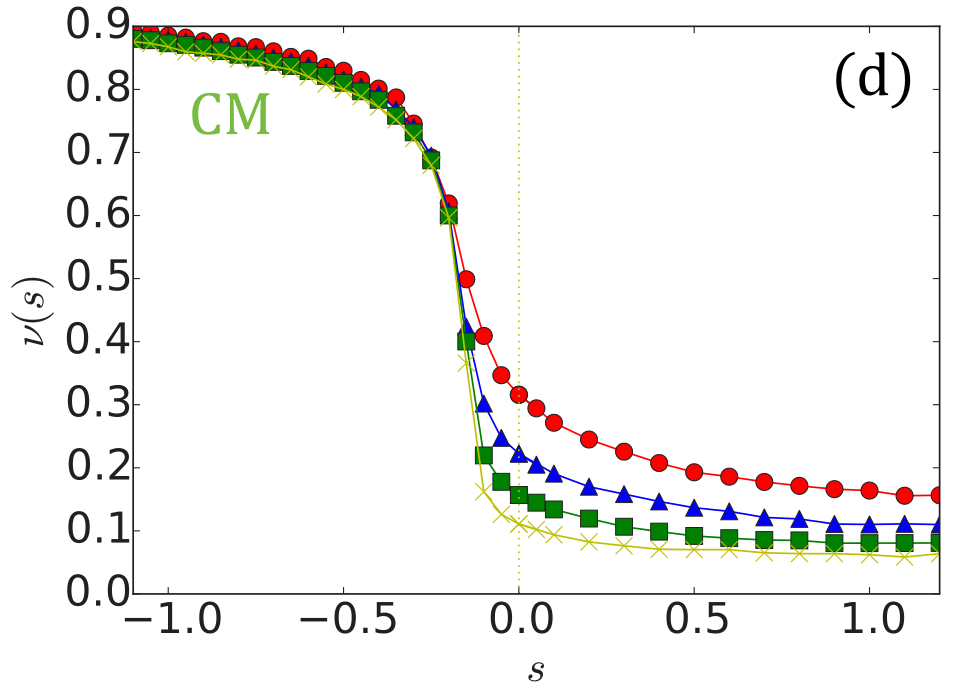
\includegraphics[width=0.49\textwidth]{Nemoto_2019_fig3d.png}
\caption{Biased average of global order parameter $\nu(s) = \left<\nu\right>_s$. $\phi = 0.65$. {\bf (a)} $l_p/\sigma = 40$ {\bf (d)} $l_p/\sigma = 6.7$. \FigureFrom{nemoto2019optimizing}{}}
\end{figure}

\begin{itemize}
  \item[$\rightarrow$] Yet there is evidence that this locus may be affected by $l_p/\sigma$!
\end{itemize}

\end{frame}

\begin{frame}{Significance of the locus of the CM transition}

% We have that the emerging picture is that there exists $s^*$ such that
% \begin{align*}
%   \left<\nu\right>_s > 0 \Leftrightarrow s < s^*
% \end{align*}
% in the limit $N \rightarrow \infty$.
%
% \return
% \begin{itemize}
%   \item[$\rightarrow$] It is unclear however if $\forall l_p/\sigma,~ s^* = 0$ or $s^* < 0$.
%   % \pause
%   \begin{itemize}
%     \item[$\rightarrow$] In the first case, this would mean that an increase of the active work above its mean value has to be accompanied with a breaking of symmetry and a global alignment of the particles in the system.
%     % \pause
%     \item[$\rightarrow$] In the second case, this would mean that there exists a way to increase the active work without aligning the particles.
%   \end{itemize}
% \end{itemize

\begin{figure}
\centering
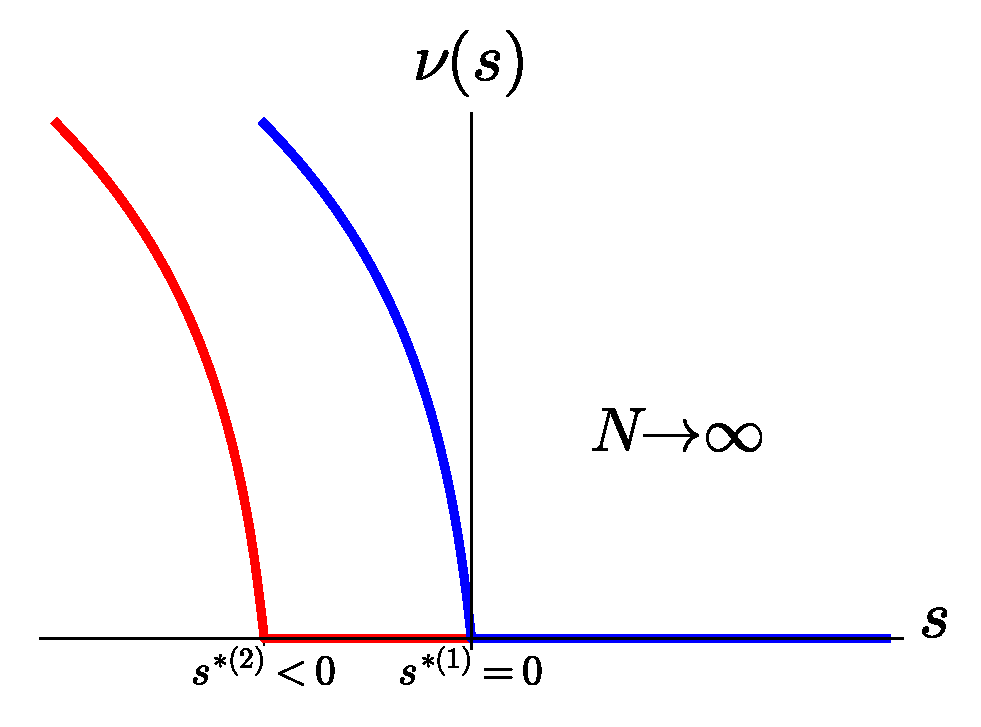
\includegraphics[width=0.6\textwidth]{nus.eps}
\end{figure}

\begin{itemize}
  \item[$\Rightarrow$] Important to disentangle active work and the coupling of orientation, and to understand the relation between them.
\end{itemize}

\end{frame}

\begin{frame}{Evidence for a CM transition at finite $s^*$}

\begin{figure}
\centering
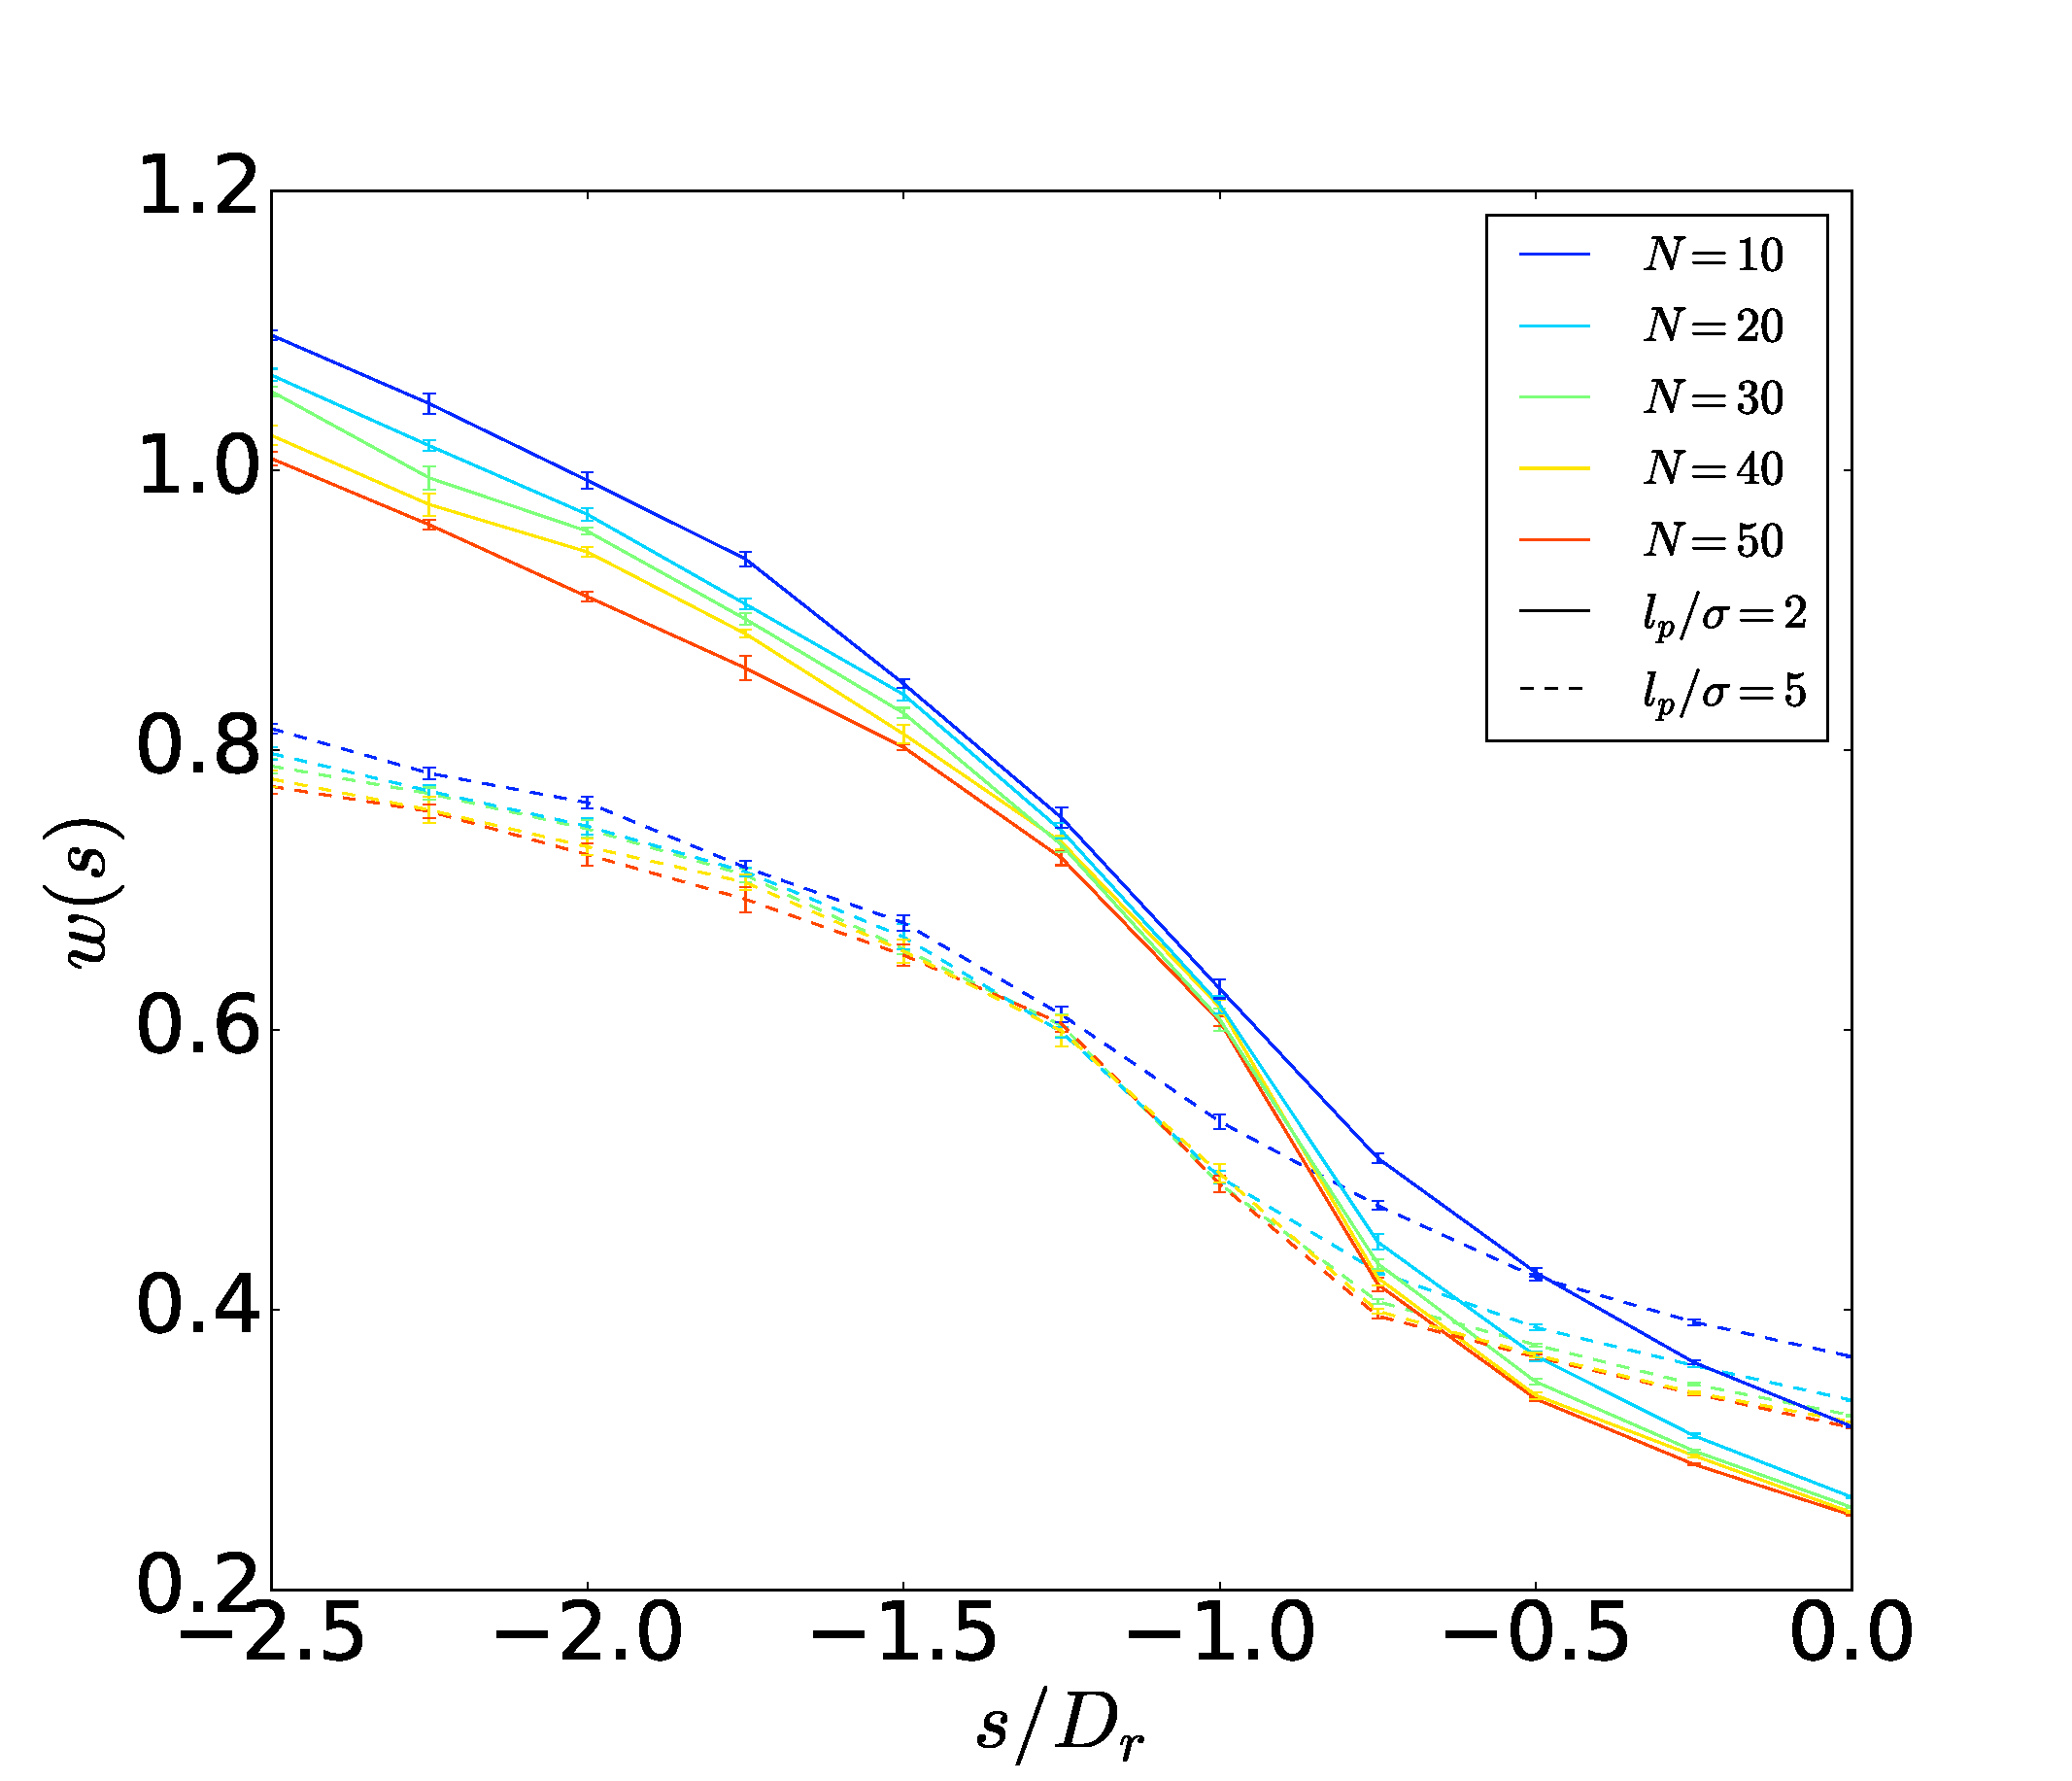
\includegraphics[width=0.49\textwidth]{sWorkN.eps}
\hfill
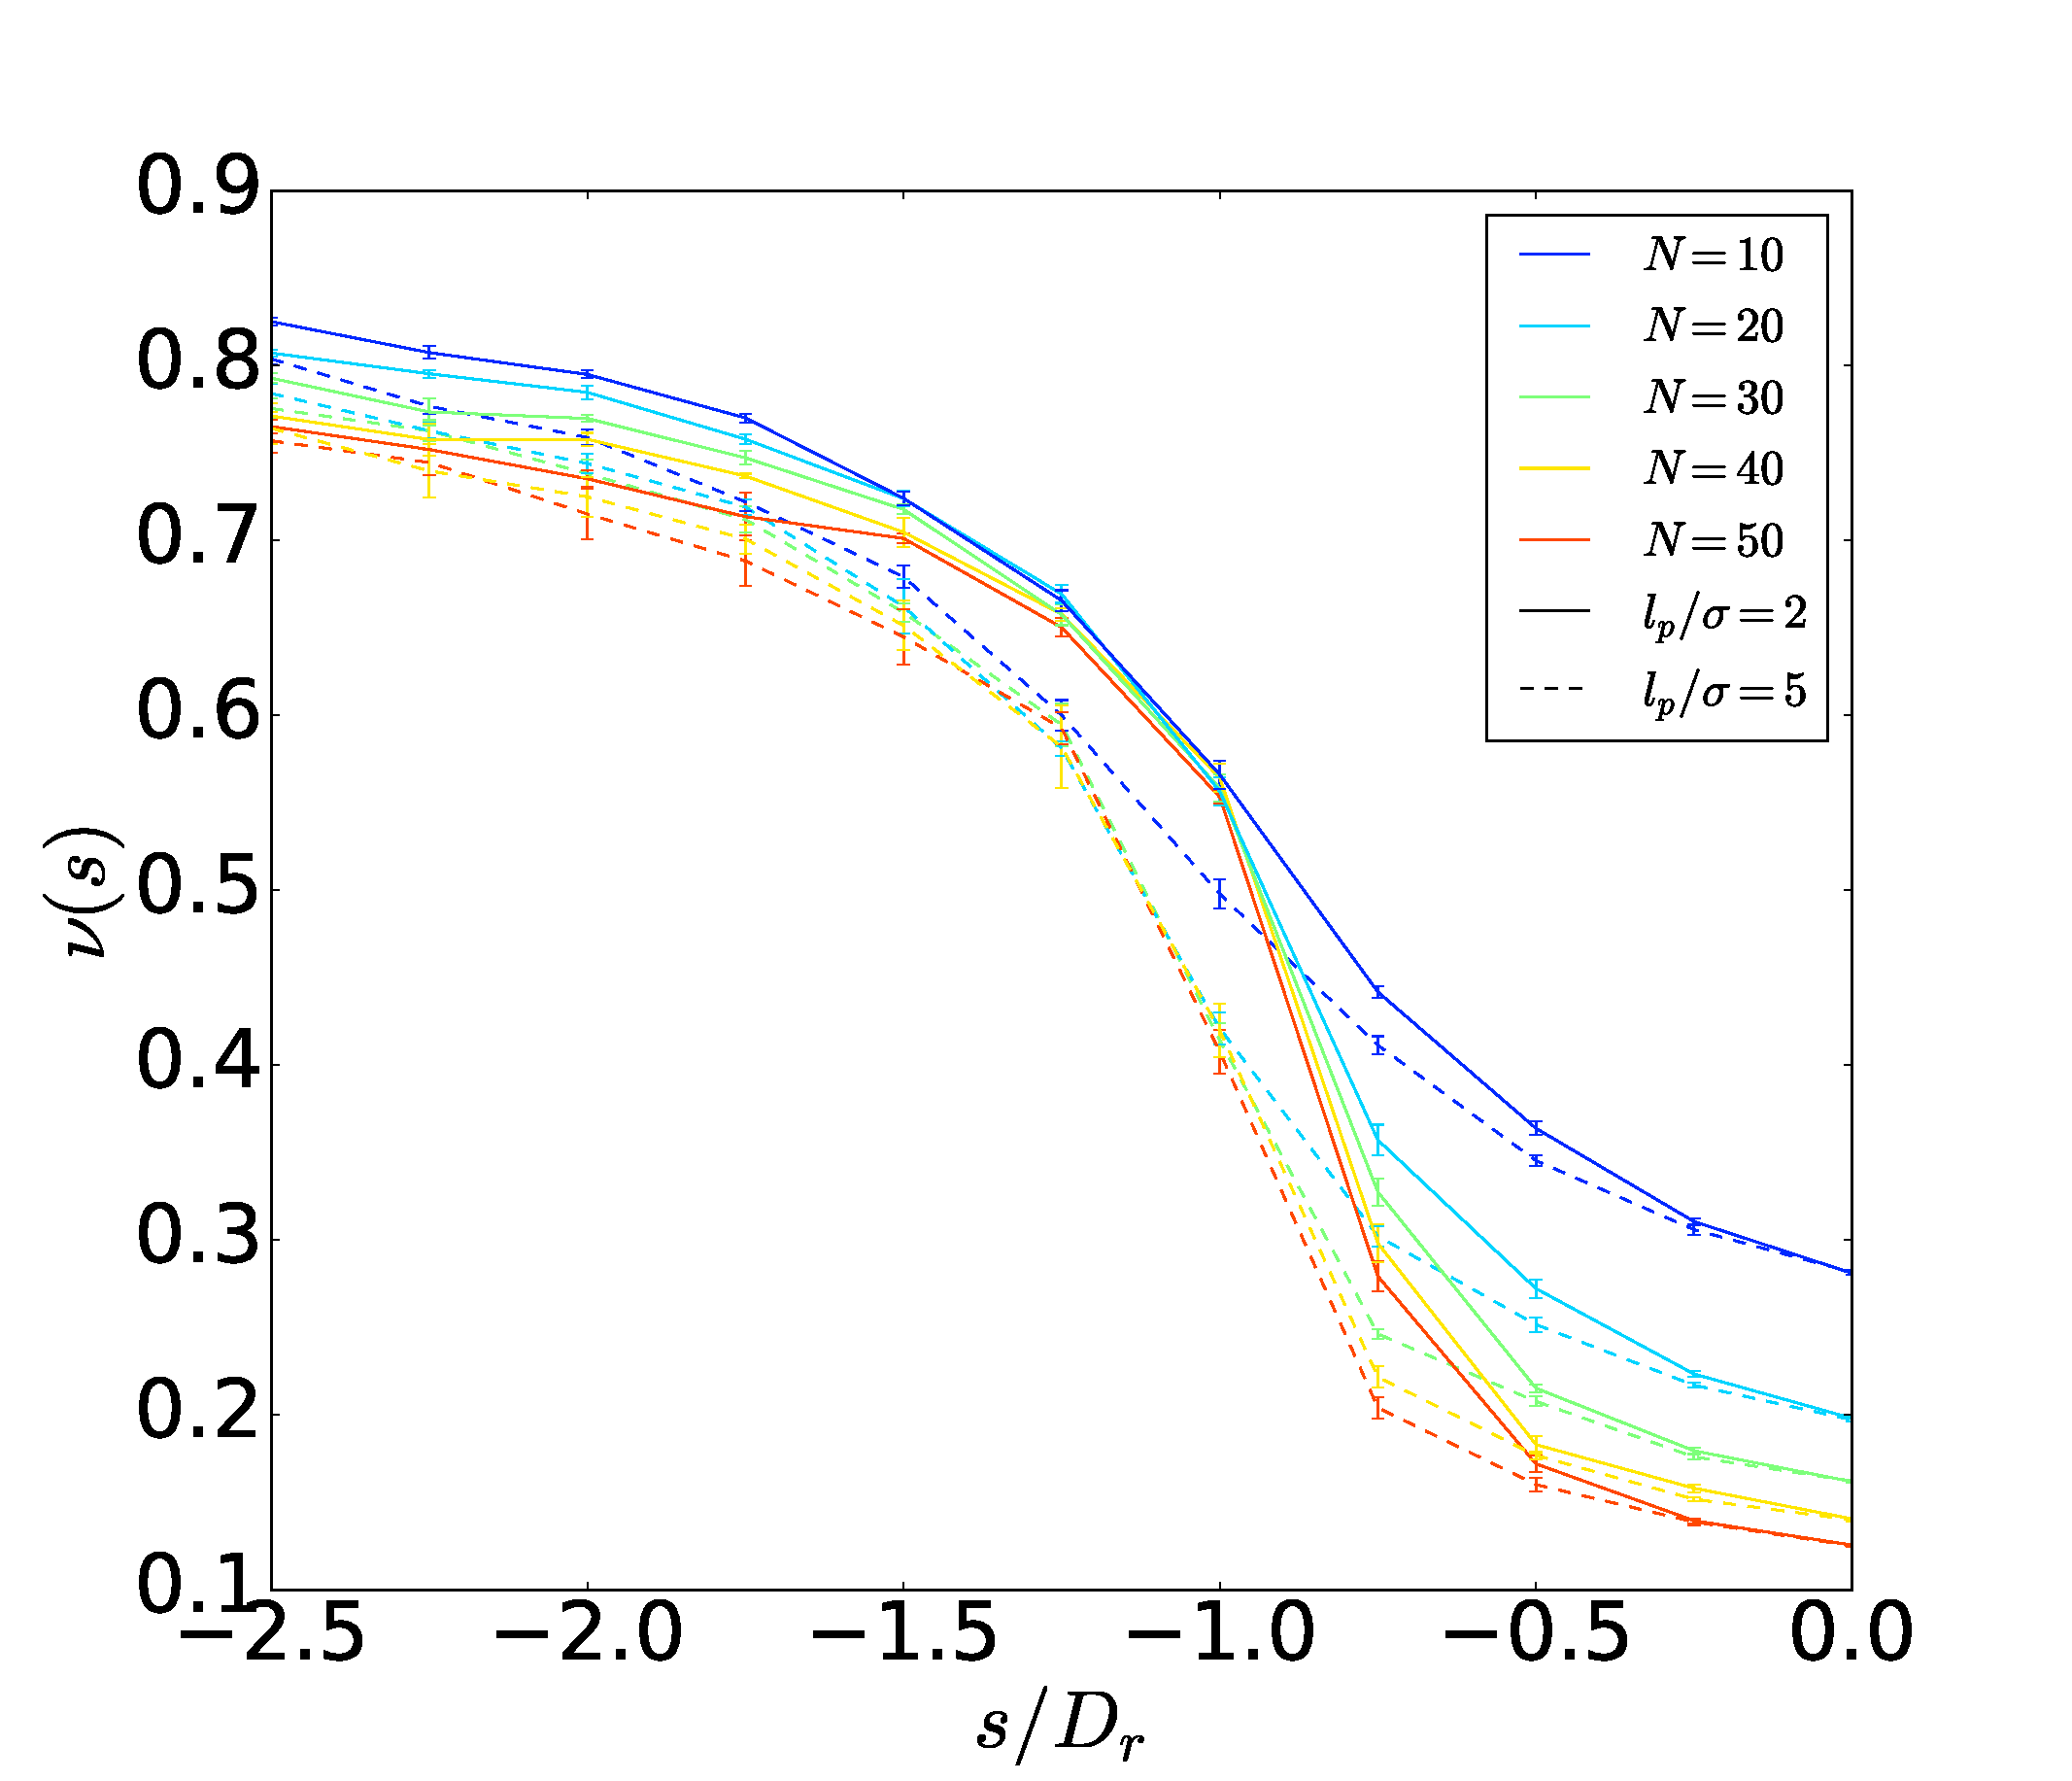
\includegraphics[width=0.49\textwidth]{sOrderN.eps}
\caption{$\phi = 0.65$, $n_c = 10^2$, $t_{\text{obs}} = 10^2$. $D_r^{-1} = l_p/\sigma$. {\bf (left)} Biased average of active work. {\bf (right)} Biased average of the global order parameter.}
\end{figure}
\begin{align*}
  s^* \approx -(l_p/\sigma)^{-1}
\end{align*}

\end{frame}

\subsection{Brownian rotors}

\begin{frame}{Independent Brownian rotors}

% In order to understand how the coupling between orientations can affect the locus of the transition we turn to the study of the independent Brownian rotors.

\begin{itemize}
  \item[$\rightarrow$] $N$ independent Brownian rotors
  \begin{align*}
  \dot{\theta}_i = \sqrt{2 D_r} \xi_i,
  \end{align*}
  which trajectories we bias with respect to
  \begin{align*}
  \epsilon_{\tau}[f] = \frac{1}{\tau} \int_0^{\tau} f(\nu(t)) \, \text{d}t.
  \end{align*}
\end{itemize}

\return
\begin{align*}
  \epsilon_{\tau}[f] \equiv \text{mean energy of microstates (trajecories)}
\end{align*}
% Recall that, in the large deviations formalism, $\epsilon_{\tau}[f]$ is equivalent to the mean energy of microstates (trajecories) $\Rightarrow$ the choice of $f$ amounts to a choice of coupling between the rotors.

% \return
% \begin{itemize}
%   \item[$\rightarrow$] Our goal is to semi-analytically derive a bound to the SCGF for these trajectories.
% \end{itemize}

\end{frame}

\begin{frame}{Choice of the bias}

\begin{align*}
  \epsilon^{(1)}_{\tau} &= \frac{1}{\tau} \int_0^{\tau} \nu(t) \, \text{d}t = \frac{1}{N\tau} \int_0^{\tau} \sum_{i=1}^N \cos(\theta_i(t) - \varphi(t)) \, \text{d}t\\
  &\approx  \frac{1}{N\tau} \int_0^{\tau} \sum_{i=1}^N \cos(\theta_i(t)) \, \text{d}t
\end{align*}
\begin{itemize}
  \item[$\Rightarrow$] Coupling to an external field.
\end{itemize}

\pause
\return
\begin{align*}
  \epsilon^{(2)}_{\tau} = \frac{1}{\tau} \int_0^{\tau} \nu^2(t) \, \text{d}t = \frac{1}{N^2\tau} \int_0^{\tau} \sum_{i,j=1}^N \cos(\theta_i(t) - \theta_j(t)) \, \text{d}t
\end{align*}
\begin{itemize}
  \item[$\Rightarrow$] Coupling between each couples of rotors.
\end{itemize}

\footnotenomark{$\theta_i$ relax significantly faster than $\varphi$ when $N \rightarrow \infty$ $\Rightarrow$ $\varphi$ treated as fixed external parameter.}

\end{frame}

\begin{frame}{Tilted generator}

\begin{align*}
\frac{\partial}{\partial t} P[\{\theta_i\}] = D_r \sum_{i=1}^N \frac{\partial^2}{\partial \theta_i^2} P[\{\theta_i\}] = \mathcal{L} P[\{\theta_i\}] \equiv \text{Fokker-Planck equation}
\end{align*}

\return
\begin{align*}
N \psi_{N,f}(s) = \lim_{t \rightarrow \infty} \frac{1}{\tau} \log\left<e^{- s N \tau \epsilon_{\tau}[f]}\right>
\end{align*}
\begin{align*}
\mathscr{W}_{s, f} = \mathcal{L} - s N f(\nu) \equiv \text{tilted generator},~ \mathscr{W}_{s, f} P[\{\theta_i\}] = N \psi_{N,f}(s) P[\{\theta_i\}]
\end{align*}

\return
\begin{align*}
\psi_{N, f}(s) = \frac{1}{N} \sup_{P} \frac{\int \text{d}^N\{\theta_i\} \, P[\{\theta_i\}] \mathscr{W}_{s, f} P[\{\theta_i\}]}{\int \text{d}^N\{\theta_i\} \, P[\{\theta_i\}] P[\{\theta_i\}]}
\end{align*}

\footfullcitenomark{touchette2018introduction}
\footfullcitenomark{jack2019ergodicity}

\end{frame}

\begin{frame}{Ansatz for the joint distribution of orientations}

\begin{align*}
P[\{\theta_i\}] \propto \exp\left(h(s) \sum_i \cos\theta_i\right) \equiv \text{distribution ansatz}
\end{align*}

\return
\begin{align*}
\psi_{N, f}(s) \geq \frac{1}{N} \sup_{h(s) \in \mathbb{R}} \frac{\int \text{d}^N\{\theta_i\} \, P[\{\theta_i\}] \mathscr{W}_{s, f} P[\{\theta_i\}]}{\int \text{d}^N\{\theta_i\} \, P[\{\theta_i\}] P[\{\theta_i\}]} = \sup_{h(s) \in \mathbb{R}} B_{s,f}(h(s))
\end{align*}
\begin{align*}
\left<f(\nu)\right>_s \approx - \frac{\partial}{\partial s} \sup_{h(s) \in \mathbb{R}} B_{s,f}(h(s)) \equiv \text{approximate order parameter}
\end{align*}

\end{frame}

\begin{frame}{Approximate polarisation from bound to the SCGF}

\vspace{-10pt}
\begin{figure}
\begin{minipage}{0.49\linewidth}
\centering
\bf Polarisation
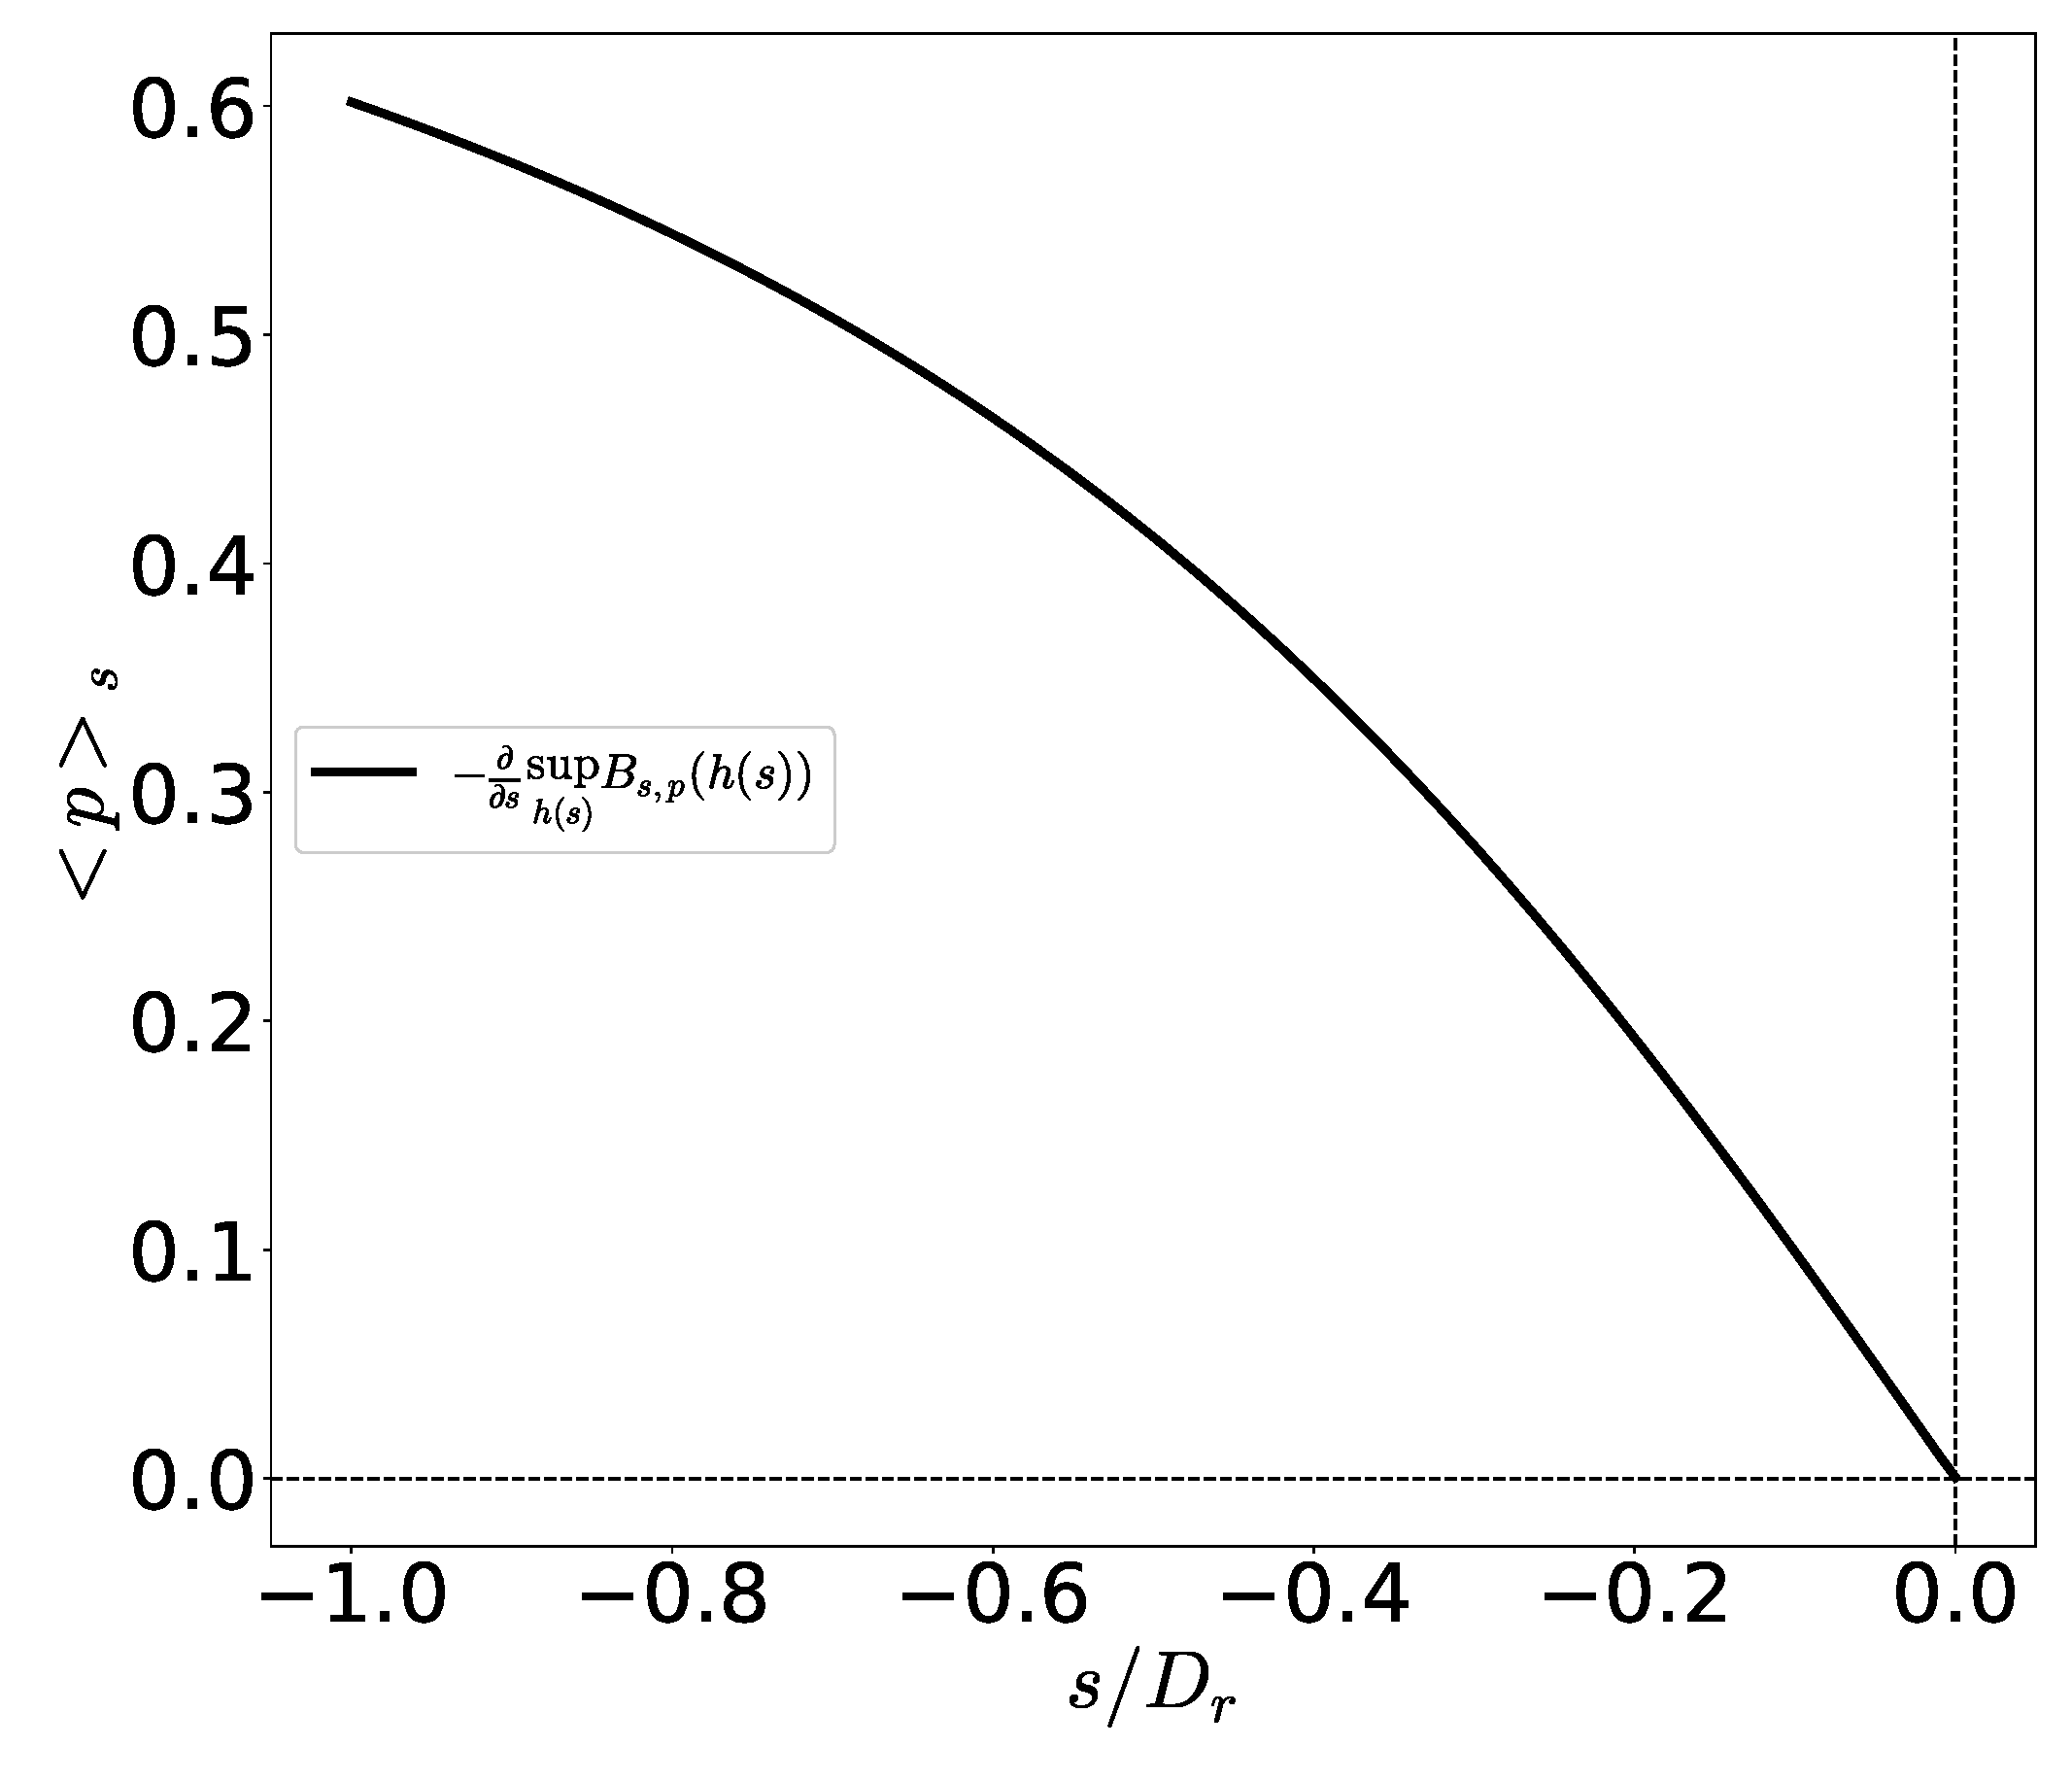
\includegraphics[width=\textwidth]{approxOrder.eps}
\end{minipage}
\hfill
\begin{minipage}{0.49\linewidth}
\centering
\bf Squared polarisation
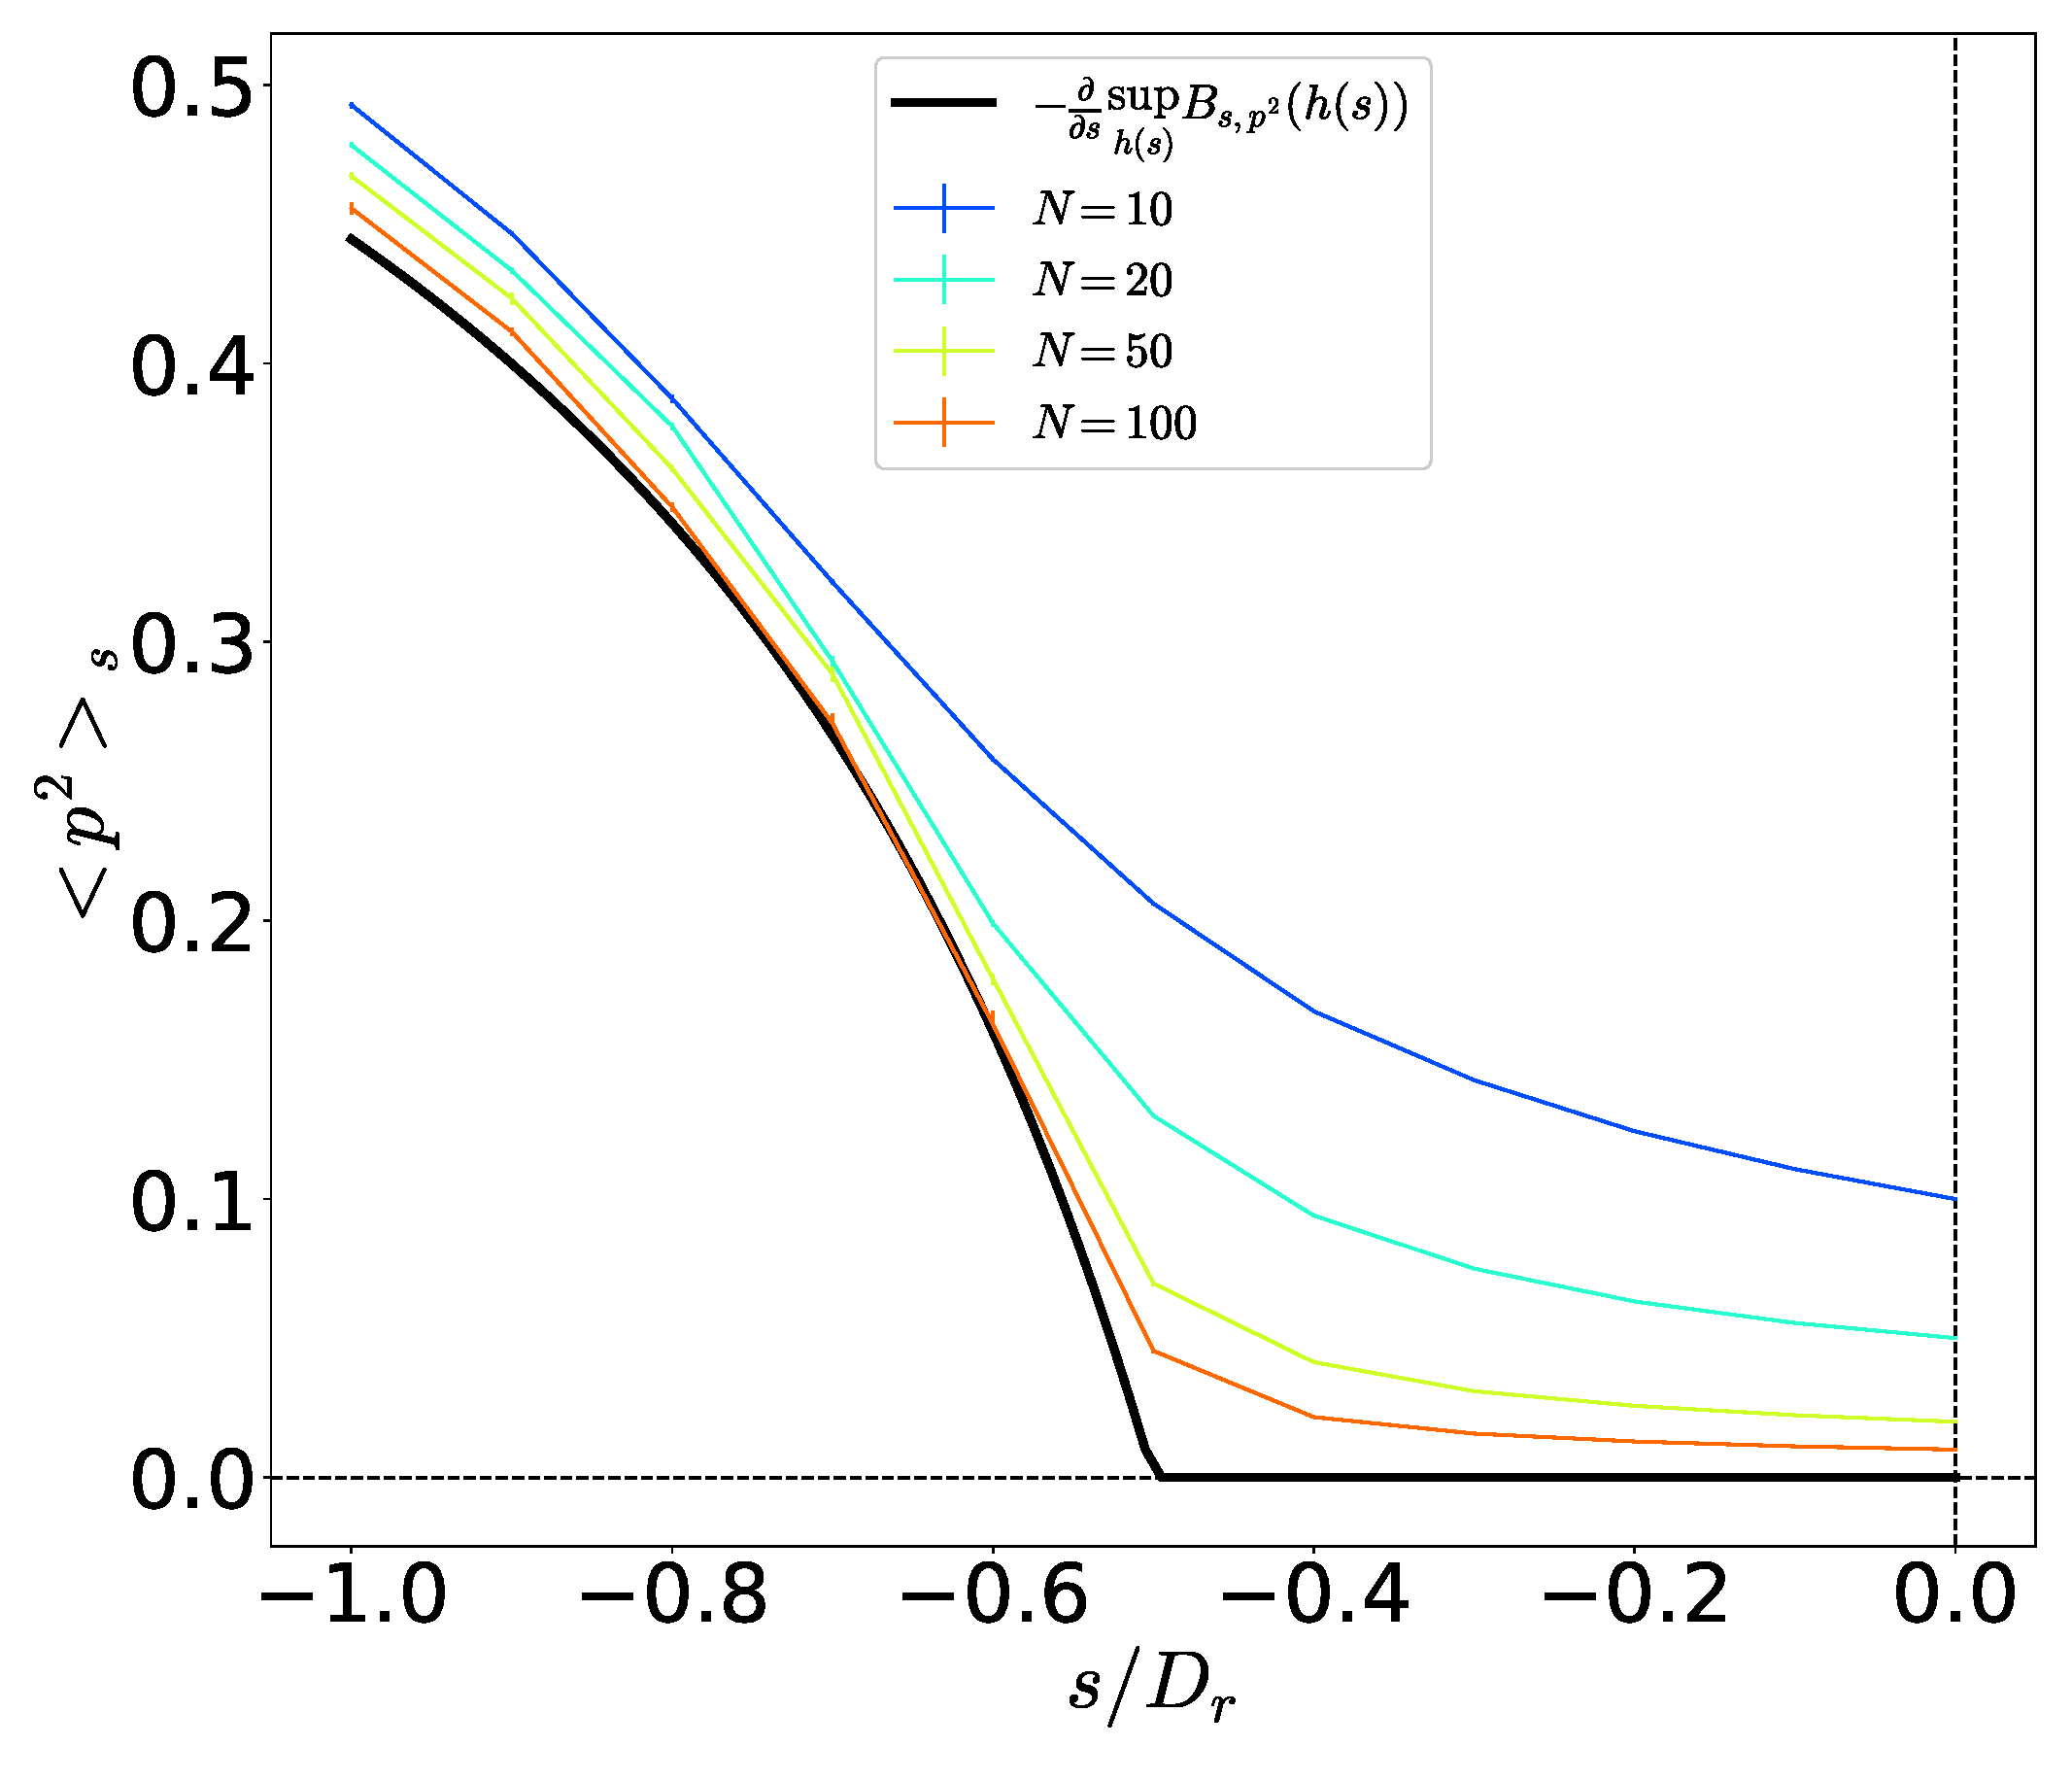
\includegraphics[width=\textwidth]{approxOrderSq_numerics.eps}
\end{minipage}
\caption{{\bf (left)} Biasing with respect to polarisation. {\bf (right)} Biasing with respect to squared polarisation. Numerical results from cloning with $n_c = 10^3$, $t_{\text{obs}} = 10^2$.}
\end{figure}

% \begin{itemize}
%   \item[$\rightarrow$] A finite $s^*$ is recovered when biasing with respect to the squared polarisation.
%   \only<1>{
%   \begin{itemize}
%     \item[$\rightarrow$] One may think of coupled Ising spins having finite magnetisation for any finite field, whereas spin coupling has to exceed thermal excitation at zero applied field.
%   \end{itemize}
%   }
%   \only<2>{
%   \begin{itemize}
%     \item[$\Rightarrow$] Back to ABPs we can hypothesise that biasing with respect to the active work is related to biasing with respect to the squared polarisation $\rightarrow$ an explicit relation between these quantities remains to be found.
%   \end{itemize}
%   }
% \end{itemize}

\end{frame}

\section{Conclusion}

\begin{frame}[t]{Conclusion}

\pause
\begin{itemize}[<+->]
  \item Large deviation theory is a powerful theoretical tool enabling us to transpose concepts from equilibrium statistical mechanics to trajectories of non-equilibrium systems.
  \item Active work quantifies dissipation in our model system of active Brownian particles.
  \item Large negative fluctuations of the active work are associated with a transition to an arrested clustered phase.
  \item Large positive fluctuations of the active work are associated with a transition to a state with global polar order.
  \item This transition towards the CM state happens at finite biasing towards higher active work in the $N \rightarrow \infty$ limit.
  \item Study of independent Brownian rotors shows that this picture is consistent with the emergence of coupling between individual particles.
  \item An explicit link between active work and global polar order remains to be found.
\end{itemize}

\end{frame}

%% THANK YOU

{
\footerwithoutframenumber
\begin{frame}[noframenumbering]

\begin{center}
\Huge
Thank you!
\end{center}

\end{frame}
}

%% SUPPLEMENTAL FRAMES

{
\footerwithoutframenumber

\begin{frame}[noframenumbering]{Contraction principle}

Consider a sequence of random variables $A_n$ satisfying a LDP with rate function $I_A$ and an other sequence $B_n = h(A_n)$\footnote{$h$ is continuous and called a contraction of $A_n$.}. We then have
\begin{align*}
  P(B_n = b) = \int_{a:h(a) = b} P(A_n = a) \, \text{d}a,
\end{align*}
therefore with Laplace's approximation we can write
\begin{align*}
  P(B_n = b) \asymp \exp\left(-n \inf_{a:h(a) = b} I_A(a)\right),
\end{align*}
which is equivalent to saying that $B_n$ satisfies a LDP with a rate function
\begin{align*}
  I_B(b) = \inf_{a:h(a) = b} I_A(a).
\end{align*}

% \pause
\return
\begin{itemize}
  \item[$\rightarrow$] Since probabilities are measured on the exponential scale, the probability of any large fluctuation should be approximated by the probability of the least improbable event leading to this fluctuation.
\end{itemize}

\end{frame}

\begin{frame}[noframenumbering]{Dissipation and structure}

\begin{figure}
\centering
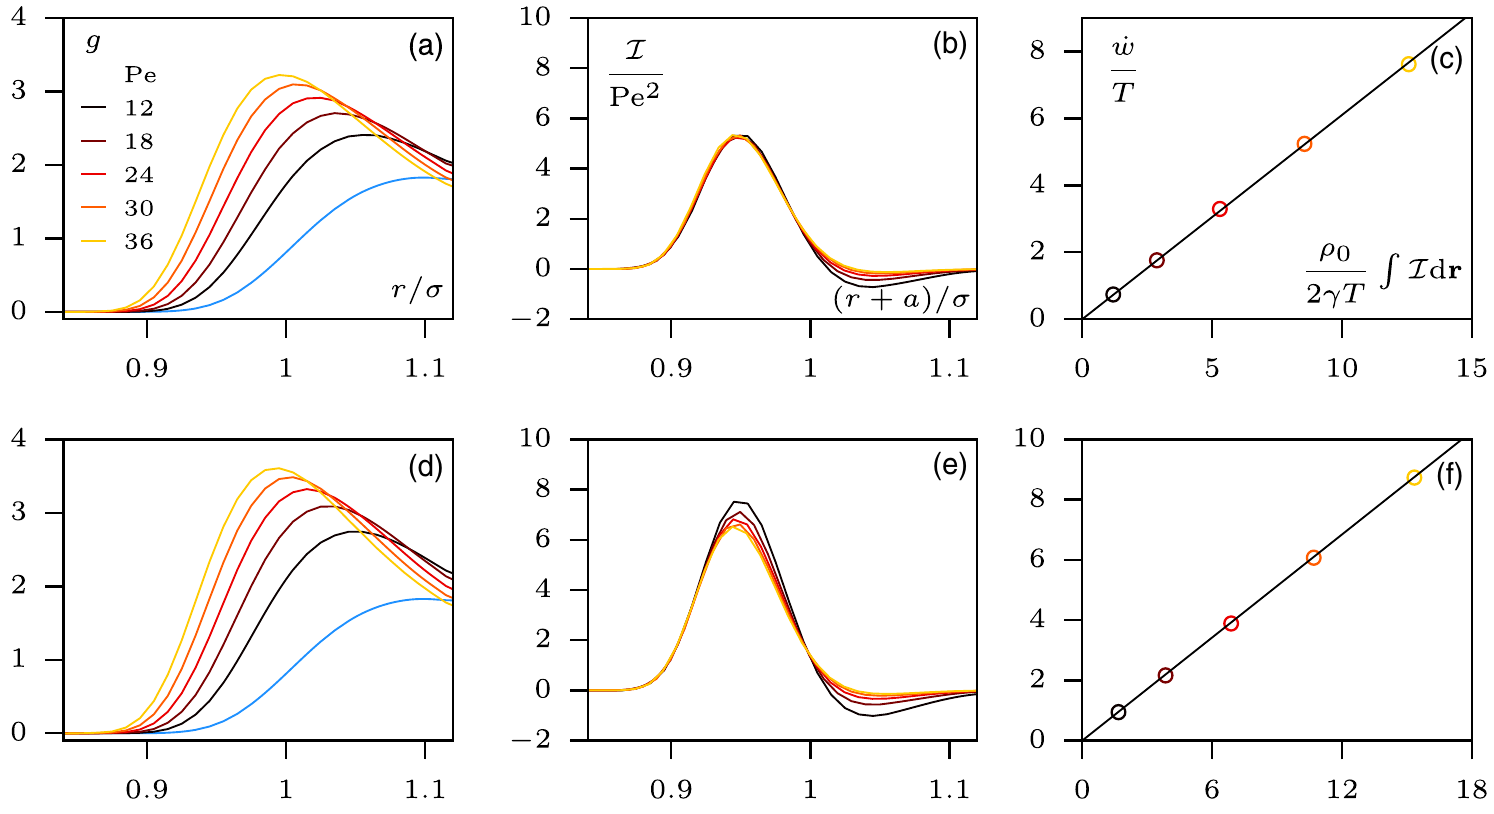
\includegraphics[width=\textwidth]{Tociu_2019_fig4.png}{}
\caption{$\dot{w} \sim -w_{f, \tau}$. $\mathcal{I} = [(\nabla v)^2 - T\nabla^2 v](g - g_{eq})$. \FigureFrom{tociu2019dissipation}{}}
\end{figure}

\end{frame}

\begin{frame}[noframenumbering]{Dissipation and transport}

\begin{figure}
\centering
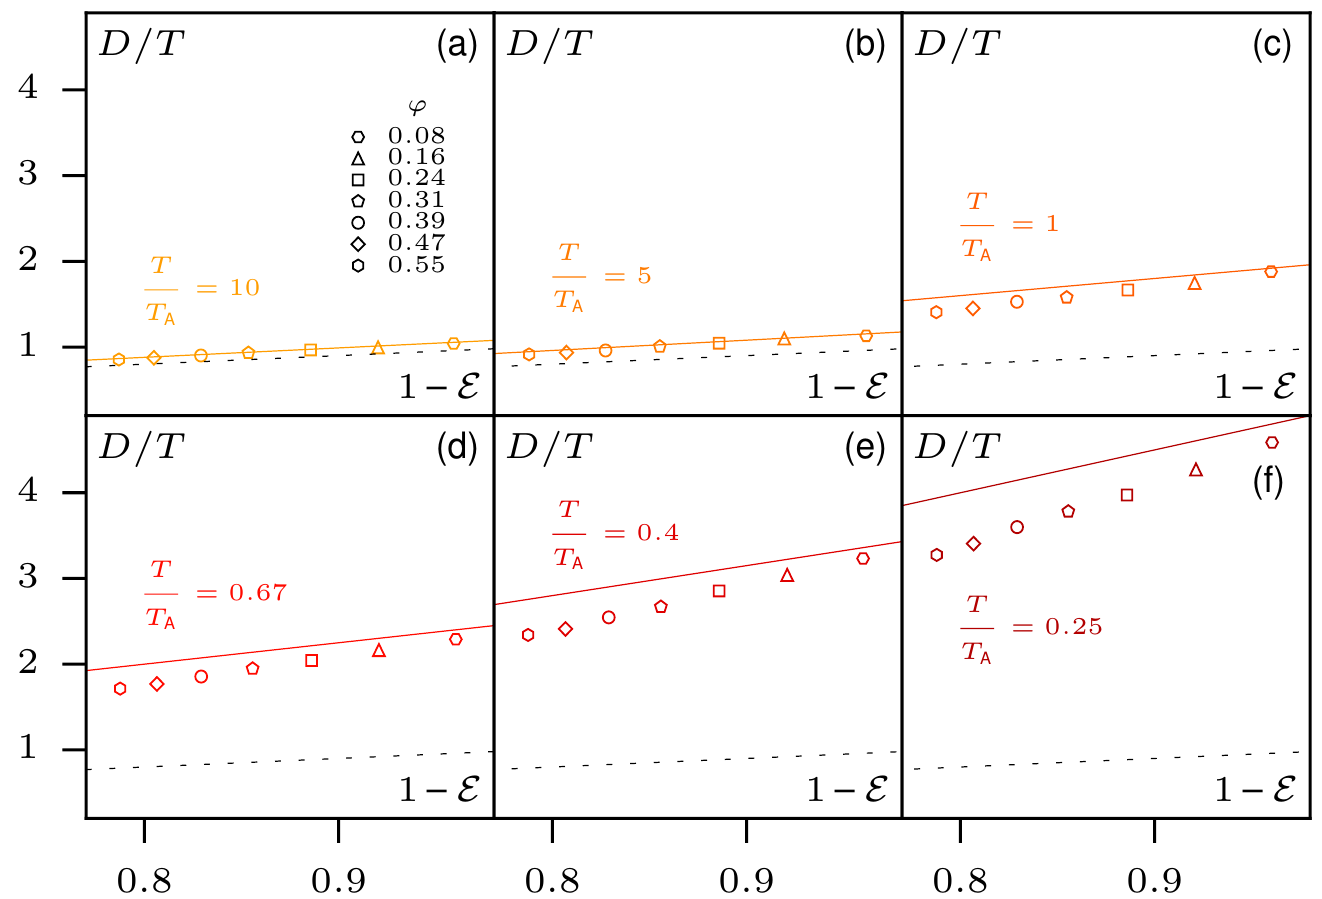
\includegraphics[width=0.8\textwidth]{Fodor_2020_fig4.png}
\caption{$1 - \mathcal{E} \sim w$. \FigureFrom{fodor2019dissipation}{}}
\end{figure}

\end{frame}

\begin{frame}[noframenumbering]{Cloning algorithm}

Consider $n_c$ copies of a system, $A_{N\tau, i}^{\beta}$ the value of observable $A_{N\tau}$ for copy $i$ on interval $[(\beta-1)\tau, \beta\tau]$, and
\begin{align*}
\Upsilon_i^{\beta} = e^{s N \tau A_{N\tau, i}^{\beta}},~ \Upsilon^{\beta} = \frac{1}{n_c} \sum_{i=1}^{n_c} \Upsilon_i^{\beta},~ \omega_i^{\beta} = \frac{\Upsilon_i^{\beta}}{\Upsilon^{\beta}},
\end{align*}
the associated weight factors. At each cloning time step $\tau$, we clone each copies $\omega_i^{\beta}$ times, so that we get the probability of observing a given trajectory with this algorithm\footfullcite{brewer2018efficient, lestang2018numerical}
\begin{align*}
P_{\text{clo}}(\{A_{N\tau, i}^{\beta}\}_{\beta=1}^{\gamma}) = P_0(\{A_{N\tau, i}^{\beta}\}_{\beta=1}^{\gamma}) \frac{\prod_{\beta=1}^{\gamma} \Upsilon_i^{\beta}}{\prod_{\beta=1}^{\gamma} \Upsilon^{\beta}} = \frac{P_s(\{A_{N\tau, i}^{\beta}\}_{\beta=1}^{\gamma})}{\prod_{\beta=1}^{\gamma} \Upsilon^{\beta}},
\end{align*}
then for $n_c \gg 1$
\begin{align*}
\prod_{\beta=1}^{\gamma} \Upsilon^{\beta} \approx \int P_s(A_{N\gamma\tau}) \, \text{d}A_{N\gamma\tau} \Rightarrow \psi_N(s, \gamma\tau) \approx \frac{1}{\gamma\tau} \sum_{\beta = 1}^{\gamma} \log \left(\frac{1}{n_c} \sum_{i=1}^{n_c} \Upsilon_i^{\beta}\right).
\end{align*}

\end{frame}

\begin{frame}[noframenumbering]{Global order rate function}

\vspace{-10pt}
\begin{align*}
  J(\overline{\nu}) = \lim_{\tau \rightarrow \infty} - \frac{1}{\tau} \log P\left(\int_0^{\tau} \nu(t) \, \text{d}t = \overline{\nu}\right),
\end{align*}
\begin{align*}
  I(w) = \inf_{\nu} I_2(w, \nu) = I_2(w, \nu(s(w))) \geq \inf_{w^{\prime}} I_2(w^{\prime}, \nu(s(w))) = J(\nu(s(w)))
\end{align*}
% \begin{itemize}
%   \item[$\rightarrow$] $J$ can be computed semi-analytically.
% \end{itemize}

\begin{figure}
\centering
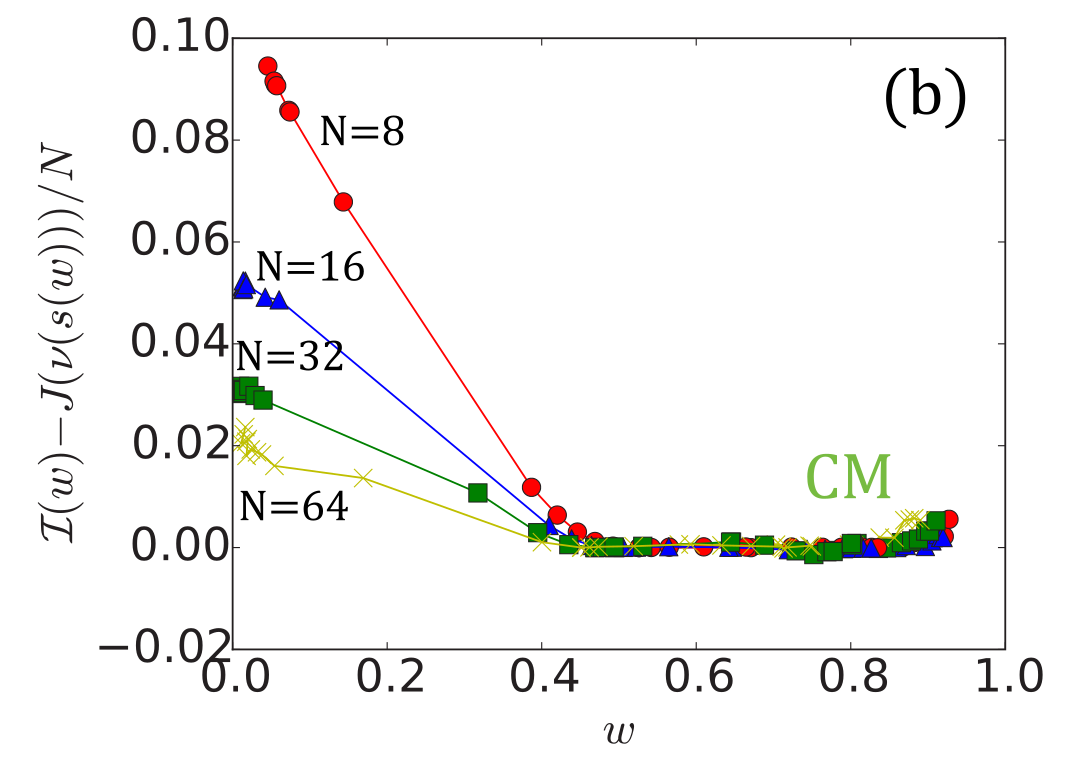
\includegraphics[width=0.49\textwidth]{Nemoto_2019_fig2b.png}
\caption{Difference of rate functions of active work and corresponding global order parameter. $\phi = 0.65$, $l_p/\sigma = 40$. We recall $\left<w\right>_0 \approx 0.4$ -- $0.45$. \FigureFrom{nemoto2019optimizing}{}}
\end{figure}

\end{frame}

}

\end{document}
